\documentclass[english]{beamer}

\usepackage{font/ubuntu}  

\usepackage{calc}

%%% Typesetting code

\usepackage{listings}


%%% Typesetting IPA

\usepackage{tipa}


%%% Vietnamese support

\usepackage{polyglossia} 
\setmainlanguage[variant=british]{english} % Should appear before biblatex if used
\setotherlanguage{vietnamese}

\newfontfamily\vietfont[Ligatures=TeX]{Linux Libertine O}
\newfontfamily\ttnocol[Ligatures=TeX]{Latin Modern Mono}


%%% Bibliography

\usepackage{biblatex}
\bibliography{biblio}
\robustify\bfseries


%%% Easy quotes

\usepackage{dirtytalk}


%%% Font management

\usepackage{fontspec}


%%% Proper math rendering
% template does not define math font! 
\usepackage{unicode-math}

%%% Verbatim management

\usepackage{verbatim}

\makeatletter
\newcommand{\verbatimfont}[1]{\def\verbatim@font{#1}}%
\makeatother

%%% Better self references

\usepackage{fancyref}


%%% Several colors by name

\usepackage{xcolor, graphicx}


%%% Pretty print numbers and international system units

\usepackage{siunitx}


%%% Extra math symbols

\usepackage{amssymb}


%%% Table stuff

\usepackage{tabularx, multirow, booktabs, colortbl}


%%% Pretty print logos of different TeX* projects

\usepackage{hologo}


%%% Hyperref and friends

\usepackage{hyperref}
\PassOptionsToPackage{hyphens}{url}
\hypersetup{urlcolor    = blue}


%%% ZH support

\usepackage{xeCJK}
\setCJKmainfont{BabelStone Han}


%%% TIKZ and friends

\usepackage{tikz}
\usetikzlibrary{positioning, fit, arrows.meta, patterns, decorations.shapes, mindmap,shadows}
\usepackage{forest}


%%% For the TIKZ mind map

\newcommand*{\info}[4][16.3]{%
  \node [ annotation, #3, scale=0.65, text width = #1em,
          inner sep = 2mm ] at (#2) {%
  \list{$\bullet$}{\topsep=0pt\itemsep=0pt\parsep=0pt
    \parskip=0pt\labelwidth=8pt\leftmargin=8pt
    \itemindent=0pt\labelsep=2pt}%
    #4
  \endlist
  };
}


%%% Larger \beamergotobutton

\renewcommand{\insertgotosymbol}{\footnotesize $\blacktriangleright$~}
\setbeamertemplate{button}{\tikz
  \node[
  inner xsep=2pt,
  inner ysep=2pt,
  draw=structure!80,
  fill=structure!50,
  rounded corners=4pt]  {\footnotesize \insertbuttontext};}


%%% Frame added before each section

\AtBeginSubsection[]{                              
  \frame<handout:0>{
    \frametitle{Outline}
    \tableofcontents[currentsection,currentsubsection]                   % Highlight current section/subsection
  }
}


%%% For better itemize lists

\let\olditem\item
\let\sitem\item%
\renewcommand{\item}{\setlength{\itemsep}{\fill}\olditem}                             
\newcommand*\elide{\textup{[\dots]}}

\newenvironment{sitemize}{\let\item\olditem \begin{itemize}}{\vfill\end{itemize}}

%%% Shading texttt

\let\textttt\texttt
\renewcommand{\texttt}[1]{\colorbox{gray!10}{\textttt{#1}}}

%%% Extra acknowledgment for the title

\makeatletter         
\newcommand{\acknowledgment}{\@dblarg\beamer@acknowledgment}  %this is where we are cloning the \title macro 
\long\def\beamer@acknowledgment[#1]#2{%
  \def\insertacknowledgment{#2}%
  }

\defbeamertemplate*{navigation symbols}{}  %remove navigation symbols



\defbeamertemplate*{footline}{}{
    \ifnum\c@framenumber=1
    \leavevmode%
    \vskip-10pt%
    \begin{beamercolorbox}[wd=\paperwidth,dp=7pt,center,colsep=0pt,sep=0pt]{ack}%
        \scriptsize\color{gray}\insertacknowledgment%
    \end{beamercolorbox}%
    \vskip0pt%
    \fi
}
\makeatother

%%% Document information 

\titlegraphic{\includegraphics[width=2cm]{images/by.eps}
}

\title{*\TeX \& gnuplot cookbook}
\subtitle{}
\author{Daniel Torregrosa \\ {\scriptsize \texttt{daniel.torregrosa @ insight-centre.org}}}
\date[\today]{\today}
\acknowledgment{If you find any mistakes, or want to add something to the slides, feel free to get in touch with me.}

%%% Start of dcument

\begin{document}


\begin{frame}
    \titlepage
\end{frame}

\begin{frame}{Contents}
\begin{enumerate}
    \item History
    \item Why use it?
    \item Basics
    \item Recipes
\end{enumerate}
\end{frame}

\begin{frame}{Disclaimer}
    \begin{itemize}
        \item The main objective is to show what \TeX{} and \texttt{gnuplot} are capable of
        \item Keep the slides as reference for later
        \item Ask at any time
    \end{itemize}
\end{frame}

\section{*\TeX}
\subsection{Introduction}


\begin{frame}{\only<2>{高德納 (Gāo dé nà)}\only<3>{Donal Knuth}}
\begin{columns}
    \begin{column}{0.5\textwidth}
    \only<3>{
        \begin{itemize}
            \item Writer of \emph{The Art of Computer Programming}
            \item Popularised big-O notation
            \item Defined literary programming
        \end{itemize}
    }
    \end{column}
    \begin{column}{0.5\textwidth}
        \centering
        \resizebox{\linewidth}{!}{
            \includegraphics{images/541px-Donald_Knuth_DSC00624.jpg}
        }
        \scriptsize{\url{https://fr.wikipedia.org/wiki/Fichier:Donald_Knuth_DSC00624.jpg}}

    \end{column}
    \end{columns}
\end{frame}

\begin{frame}{The Art of Computer Programming}
    \begin{itemize}
        \item The first volume of \emph{The Art of Computer Programming} was published in 1968 using hot metal typesetting
        \only<2>{{
            \centering
            \resizebox{\linewidth}{!}{
                \includegraphics{images/Matrixcase-bembo-16pts.jpg}
            }}
        }
        \only<3> {
            \item In 1977, Knuth found the phototypeset galley proofs for the second volume inferior, as hot metal typesetting had fell out of use
            \item Unhappy with both typesetting and fonts, he \dots{}
        }
    \end{itemize}
\end{frame}

\begin{frame}{\TeX{} history}
    \begin{itemize}
        \item In 1977, Knuth writes a memo describing \TeX
        \item In 1978, a first version of \TeX{} was implemented in \texttt{SAIL}
        \item In 1982, \TeX{}82 (sometimes \TeX{}\texttt{2.0}) became Turing complete
        \item In 1984, the \TeX{}book instructs the reader to pronounce \TeX{} as \textipa{/t3x/}, from τέχνη
        \begin{sitemize}
            \item \say{It's the \textit{ch} sound in Scottish words like \textit{loch} or German words like \textit{ach}; it's a Spanish \textit{j} and a Russian \textit{kh} [Х]} \textit{Donal Knuth, \TeX{}book, 1984}
        \end{sitemize}
        \item In 1989, \TeX{} \texttt{3.0} became \emph{ready to use} (feature frozen)
    \end{itemize}
\end{frame}

\begin{frame}{\TeX{} \texttt{3.0} features}
    \begin{itemize}
        \item Turing complete
        \item Macro and token based language
        \item Expansion of macros is almost side-effect free
        \item Tail recursion makes it very efficient
        \item Written in WEB, that combines \TeX{} and a subset of Pascal
        \begin{itemize}
            \item See \textit{\TeX: The Program}
        \end{itemize}
    \end{itemize}
\end{frame}

\begin{frame}{\hologo{METAFONT}}
    \begin{itemize}
        \item Makes fonts from strokes with finite-width pens and filled regions
        \item Computer Modern is the most famous example {\fontfamily{cmr}\selectfont(also the default font in \TeX{})}
        \item Produces typefaces (rasterised glyph)
        \item Mostly superseded by vector-based font systems (e.g. Postscript, TrueType, OpenType)
        \item \say{\ldots asking an artist to become enough of a mathematician to understand how to write a font with 60 parameters is too much.} \textit{Donald E. Knuth, 1996}
    \end{itemize}
\end{frame}

\begin{frame}{Other trivia}
    \begin{itemize}
        \item The \textit{Device independent file format} (DVI) was designed by David Fuchs and implemented by Knuth; 
        \begin{sitemize}
            \item \TeX{} outputs \texttt{.dvi} files
            \item Mostly superseded by postscript, a turing-complete stack-based format developed by Adobe to communicate with printers
        \end{sitemize}
        \item \say{At the time of my death, it is my intention that the then-current versions [\ldots] should become \TeX, Version $\pi$ and \hologo{METAFONT}, Version $e$, respectively. From that moment on, all \say{bugs} will be permanent \say{features.}} \textit{Donal Knuth, The future of \TeX{} and \hologo{METAFONT}, 1990}
    \end{itemize}
\end{frame}

\subsection{Rationale}
\begin{frame}{Why *\TeX}
    \begin{itemize}
        \item Content/presentation split
        \item Typesetting math
        \item Automatising: no need to typeset half the document because you added a new figure
        \item Reference management via \hologo{BibTeX}
        \item Design: can you compete with the combined contributions of hundreds of developers extremely passionate about design over 30 years?
    \end{itemize}
\end{frame}

\begin{frame}[fragile]{Why not *\TeX}
    \begin{itemize}
        \item {WYSIWYG editors require almost no skills or knowledge, producing \textit{good enough} output}
        \item Hard to find answers to some problems because they can be easily done in an incompatible way (specially \hologo{XeTeX} and \hologo{LuaTeX} specific solutions)
        \item 30 years of development left a lot of waste 
        \item Sometimes \LaTeX is very obtuse in the way it works %Intentional lack of {}
        \begin{sitemize}
            \item \texttt{Overfull \textbackslash{}hbox (21.67pt too wide)}
            \item Position of floats
            \item Use of \verb|\fragile| and \verb|\robust|
            \item \verb|\makeatletter|
        \end{sitemize}        
    \end{itemize}
\end{frame}

\begin{frame}{Corollary }
    \begin{itemize}
        \item \TeX{} is a typesetting program, not a program for typesetting
        \item WYSIWYG editors are programs for typesetting
        \begin{sitemize}
            \item Arguably, libreoffice-like editors are quite bad at it
            \item inkscape-like programs should be used for proper typesetting
        \end{sitemize}
    \end{itemize}
\end{frame}

\subsection{Basics}
\label{sec:basics}

\begin{frame}[fragile]{\TeX }
\begin{itemize}
    \item \TeX{} undergone a feature freeze in 1989
    \item \TeX{} is a typesetting \textit{engine} with primitives 
    \item \TeX{} is also a binary that takes \TeX{} files and outputs \texttt{.dvi}
    \item Over the years, different engines were developed:
    \begin{sitemize}
        \item \hologo{eTeX}, that improved \TeX{} significantly
        \item \hologo{pdfTeX}, that can output both \texttt{dvi} and \texttt{pdf} formats
        \item \hologo{XeTeX}\only<2>{ (\textipa{/\textprimstress{}zi:t3x/})}, with support for unicode and modern font formats(\texttt{otf}). Results are mostly faithful to \hologo{eTeX}
        \item \hologo{LuaTeX}, that exposes a secondary Lua interface for building macros. There are significant changes in how different elements are rendered (e.g. hyphenation, ligatures, etc.)
    \end{sitemize}
    {\small See \url{https://tex.stackexchange.com/questions/222286/what-are-the-incompatibilities-of-pdftex-xetex-and-luatex}}
\end{itemize}
\end{frame}

\begin{frame}{Distribution files}
\begin{itemize}
    \item Distribution files (\texttt{ltx} extension) provide several macros to ease working with \TeX{}
    \item Plain \TeX{} is the simplest one
    \item \LaTeX{}, started by Leslie Lamport, is an enhanced collection of macros (\textit{document preparation system}), and the most used one (currently \hologo{LaTeXe})
    \item \hologo{ConTeXt}  was developed concurrently with \hologo{LuaTeX}
    \item This document is typeset with \hologo{XeLaTeX} (\hologo{XeTeX} engine with \hologo{LaTeXe} macros)
\end{itemize}
\end{frame}

\begin{frame}{Classes and packages}
    \begin{itemize}
        \item Class
        \begin{sitemize}
            \item \texttt{.cls} extension
            \item All documents should have exactly 1 class, selected using \texttt{documentclass}
        \end{sitemize}
        
        \item Package
        \begin{sitemize}
            \item \texttt{.sty} extension
            \item Any number of packages can be included using \texttt{usepackage}
        \end{sitemize}
        
        \item Distribution (\texttt{.ltx}), classes (\texttt{.cls}) and packages (\texttt{.sty}) are all \TeX{} format files
    \end{itemize}
\end{frame}

\begin{frame}{Document classes}
    \begin{itemize}
        \item \texttt{article} for articles
        \item \texttt{book} for books
        \item \texttt{beamer} for slides
        \item Hundreds more \url{https://ctan.org/topic/class}
        \item Each one defines layouts, macros, fonts, etc.
    \end{itemize}
\end{frame}

\begin{frame}{Packages}
    \begin{itemize}
        \item Packages further extend \LaTeX{} functionality
        \item Several packages to be explored later
    \end{itemize}
\end{frame}

\begin{frame}[fragile]{Primitives}
    \begin{itemize}
        \item Tokens: just about anything not starting with \textbackslash{}
        \item Commands: anything starting with \textbackslash{}
        
        \item \hyperlink{sld_charcodes}{\beamergotobutton{More on \textbackslash{}}}
    \end{itemize}
\end{frame}

\begin{frame}[fragile]{Toggles vs macro vs environment}
    \begin{itemize}
        \item There is no real distinction between these commands! 
        \item Toggle: \verb|\centering|, \verb|{\bfseries text in bold}|
        \item Macro: \verb|\item|, \verb|\textbf{text in bold}|
        \item Environment: \verb|\begin{frame}|,
        \begin{verbatim}
\newenvironment{boldenv}%
{\bfseries}%
{}
...
\begin{boldenv} text in bold \end{boldenv}
        \end{verbatim} 
        
        
        (not by default in \LaTeX{}, \hyperlink{sld_macros}{\beamergotobutton{Defining macros}})
    \end{itemize}
\end{frame}

\begin{frame}[fragile]{Environments}
    \begin{itemize}
        \item Basically scopes
        \item \{\} delimits an environment
        \item From \textit{outside}, an \{\} delimited block is just a token
        \item \verb|\begin{myEnv}|\dots{} \verb|\end{myEnv}| implicitly creates an environment:
        \begin{sitemize}
            \item A macro with the same name (\texttt{myEnv}) that can take parameters
            \item A scoped block (the content between begin and end)
            \item A macro with the same name starting with end (\texttt{endmyEnv})
        \end{sitemize}
        \item E.g. you can call \verb|\center|, that is called where \verb|\begin{center}| is used, but will likely break the rest of the document
    \end{itemize}
\end{frame}



\begin{frame}[fragile]{Dealing with hungry macros}
    \begin{itemize}
        \item Macros usually eat the next token (usually, a space)
        % \begin{sitemize}
        %     \item Otherwise, \verb|\bfseries bold text| would not be possible without a space
        % \end{sitemize}
        \item \LaTeX{} macros also eat blocks enclosed in [] (optional parameters)
        \begin{sitemize}
            \item That is, those defined with \verb|\newcommand| instead \verb|\let| or \verb|\def|
        \end{sitemize}
        \item Sometimes \{\} is enough to stop expansion, e.g. \verb|\TeX{}| 
        \item The correct way to stop macro expansion is using \verb|\relax|
    \end{itemize}
\end{frame}

\begin{frame}[label=sld_charcodes]{Character category codes}
    \begin{tabular}{lrr|lrr}
         0 & Escape & \textbackslash{} & 1 & Begin group & \{  \\
         2 & End group & \} &  3 & Math shift & \$ \\
         4 & Alignment & \& & 5 & End-of-line & \textbackslash n \\
         6 & Parameter & \# &7 & Superscript & \textasciicircum{} \\
         8 & Subscript & \textunderscore & 9 & Ignored & \\
         10 & Space & \%20, \textbackslash{}t & 11 & Letters & abc \\
         12 & Other & 1.+ & 13 & Active character & \textasciitilde{}  \\
         14 & Comment & \% &  15 & Invalid input & \texttt{[DEL]} \\
    \end{tabular}
\end{frame}

\begin{frame}[fragile]{Other character}
    \begin{itemize}
        \item Both code 11 (letters) and 12 (other) get rendered when part of a token
        \item But, macro names can only be composed of letters
        \item \TeX{} has no namespacing mechanism
        \item Hence, we can make \textit{protected} macros by temporarily telling \TeX{} that a certain \textit{other} is now a \textit{letter}, e.g.
    \end{itemize}
        \begin{verbatim}
\makeatletter
\newcommand{@myprotectedcommand}{...}
\makeatother
...
\@myprotectedcommand

[Massive error log due to writing something unparseable]
        \end{verbatim}
\end{frame}

\begin{frame}{Active character}
    \begin{itemize}
        \item Active characters are considered commands (just like any other escaped sequence of letters)
        \item The only default active character is \textasciitilde{}, that is a non breaking space
        \item \textunderscore{} and \textasciicircum{} seem but are not active, they have its own category (7 and 8)!
        \item You can play with this, but it will bite
    \end{itemize}
\end{frame}

\begin{frame}{\only<2>{``}Variables\only<2>{''}}
    \begin{itemize}
        \item \LaTeX{} defines some variables, e.g. for keeping track of counters
        \item Some documents or packages define \only<1>{variables} \only<2>{macros} such as \texttt{author}, \texttt{title}, \texttt{subtitle}, etc.
        \only<2>{
        \item Actually, \TeX{} does not support variables at all!
        \item Done with macros, e.g. \texttt{acknowledgement} \hyperlink{sld_ack}{\beamergotobutton{defined in this document}}}
    \end{itemize}
\end{frame}

\begin{frame}[fragile]{Other common caveats}
    \begin{itemize}
        \item Should escape: \# \$ \% \& \_ \{ \} 
        \item Should use \texttt{text*} command: \textbackslash{} \textasciitilde{} \textasciicircum{}
        \item \verb|\^ \~| add accents to the next letter
        \item{} < > should be typed \verb|\textless\textgreater| 
        \begin{sitemize}
            \item unless your engine can use \texttt{UTF-8}, e.g. \hologo{XeTeX}
            \item {beamer} adds special parameters enclosed in <> for some macros
        \end{sitemize} 
        \item \verb|`'| or \verb|``''| for proper ``quotation''! \verb|"| will break documents
        \item Likewise, \verb|\cdots| for \dots{} (do not ...)
        \item \verb|--| for en--dash, \verb|---| for em---dash
    \end{itemize}
\end{frame}

\begin{frame}[fragile]{Compilation times}
    \begin{itemize}
        \item \LaTeX{} compilation is optimised by cutting some corners, ``hacky'' commands (e.g. \verb|\verb|) should only be used in \texttt{fragile} blocks (that will take longer to compile)
        \item Macros are better defined before the start of the document (or in fragile blocks)
        \item Robust macros (\verb|\robust\bfseries|) do not need to be protected with fragile (but will take longer to compile)
        \item Adding \texttt{[draft]} to the document class will make compilation faster, but images are placeholders, links do not work, etc.
        \item Multiple compilations: \LaTeX{} should be invoked multiple times, with (likely) invocations of \texttt{bibtex} and other libraries in between. Use \texttt{latexmk}, \texttt{xelatexmk}, etc. for best results
    \end{itemize}
    
\end{frame}

\begin{frame}[fragile]{Whitespace is fun}
\begin{columns}
    \begin{column}{0.5\textwidth}
\begin{itemize}
\item One or more   spaces 
will be considered 
a word delimiter
\item One line break 
will be considered 
a word delimiter too!
\item Two line breaks 

will actually break the line
\end{itemize}
    \end{column}
    \begin{column}{0.5\textwidth}
    \begin{verbatim*}
\begin{itemize}
\item One or more   spaces 
will be considered 
a word delimiter
\item One line break 
will be considered 
a word delimiter too!
\item Two line breaks 

will actually break the line
\end{itemize}
    \end{verbatim*}
    \end{column}
\end{columns}
\end{frame}

\begin{frame}[fragile]{Whitespace is fun II}
    \begin{itemize}
        \item \textasciitilde{} (active character!) represents a non-breaking space
        \begin{sitemize}
            \item E.g. \verb|Section~\ref{label}| will never put the number in the next line
        \end{sitemize} 
        \item \verb|\\| forces a line break
        \item \verb|\break| breaks the line without filling it (usually results in bad typesetting)
        \item \verb|\clearpage| and \verb|\newpage| force a page break
        \begin{sitemize}
            \item Some styles (e.g. book) offer a \verb|\newoddpage| command
        \end{sitemize} 
        \item Spaces (\verb|\vspace{10pt}|, \verb|\hspace{2ex plus 1ex minus 1ex}|) add a fixed space
        \item Skips are predefined spaces, e.g. \verb|\smallskip|
        \item Fills (\verb|\vfill|, \verb|\hfill|) take all the free space
    \end{itemize}
\end{frame}

\begin{frame}[fragile]{Sectioning}
    \begin{itemize}
        \item \LaTeX{} has several sectioning depths:
        \begin{enumerate}\setcounter{enumi}{-2}
            \sitem \verb|\part|
            \sitem \verb|\chapter|
            \sitem \verb|\section|
            \sitem \verb|\subsection|
            \sitem \verb|\subsubsection|
            \sitem \verb|\paragraph|
            \sitem \verb|\subparagraph|
        \vfill\end{enumerate}
        \item Some only available in some classes, e.g. -1 and 0 only available in \texttt{book}
        \item Package \texttt{titlesec} can be used to configure how are they rendered
        \item Adding an * to the macro will create an unnumbered section that will not appear in the table of contents (e.g. \verb|\section*|)
        \item \verb|\tableofcontents| inserts the table of contents (and can be configured)
    \end{itemize}
\end{frame}

\begin{frame}{Macro*}
    \begin{itemize}
        \item Many packages offer macro variants that end in *, e.g. 
        \begin{sitemize}
            \item \texttt{section*}, a \texttt{section} without number
            \item \texttt{figure*}, a page-width figure in two-column documents
            \item \texttt{caption*}, a figure caption that does not start with \textbf{Figure 4:}
        \end{sitemize}
        \item But, those are macros manually defined by the different packages
        \item The * has no specific meaning, do not assume macro* always exist
    \end{itemize}
\end{frame}

\begin{frame}[fragile]{Modularity}
    \begin{itemize}
        \item \verb|\input| \textit{copies and pastes} the content of a different file in this position
        \item \verb|\include| is similar, but recursive calls are forbidden and forces a page break
        \item \verb|\includeonly| before \verb|\include| can limit the includes (for faster compilation times)
    \end{itemize}
\end{frame}

\begin{frame}{Comments}
    \begin{itemize}
        \item The character \% (character code 14) makes the parser ignore the rest of the line
        \item Beware in math mode! Incorrectly typed $100\%$ may break the document
        \item Newline can be ignored writing \% at the end of the line; this is sometimes needed when defining macros 
    \end{itemize}
\end{frame}

\begin{frame}[fragile]{Lists}
    \begin{itemize}
        \item \texttt{itemize} for unnumbered lists
        \item \texttt{enumerate} for numbered lists
        \item \verb|\renewcommand{\theenumi}{\Roman{enumi}}%| can be used for roman numbers
        \begin{sitemize}
            \item Also \texttt{arabic} (default), \texttt{roman}, \texttt{alph} and \texttt{Alph}
        \end{sitemize} 
        \item[$\rightarrow$] bullets can be replaced with (almost) anything 
        \item \texttt{description} for better management of label bullets
        \begin{sitemize}
            \item Optional \texttt{align} parameter to align labels
        \end{sitemize}
    \end{itemize}
\end{frame}

\begin{frame}[fragile]{Font sizes}
    \begin{itemize}
        \item \LaTeX{} offers several pre-defined font sizes
        \begin{center}
            \begin{tabular}{cccc}
                 \verb|\Huge| & \verb|\huge| & \verb|\LARGE| & \verb|\Large| \\
                 \verb|\large| & \verb|\normalsize| & \verb|\small| & \verb|\footnotesize|  \\
                 \verb|\scriptsize| & \verb|\tiny| & & 
            \end{tabular}
        \end{center}

        \item Other packages can add more, e.g. \texttt{beamer}'s \verb|\VERYHUGE|
        \item Whole document \textit{base} font size can be altered, e.g. \verb|\documentclass[11pt]{article}|
        \item \verb|\fontsize{size}{baselineskip}\selectfont| to choose an arbitrary size
        \item Package \texttt{anyfontsize} can be used for arbitrary sizes
        \begin{sitemize}
            \item Raster fonts might not have all sizes
            \item Vector fonts can be scaled arbitrarily
        \end{sitemize}
    \end{itemize}
\end{frame}

\begin{frame}[fragile]{Font faces}
    \begin{itemize}
        \item Usually, several predefined styles exist, e.g.
        \begin{sitemize}
            \item Bold: \verb|\textbf{}|, \verb|\bfseries|
            \item Italics: \verb|\textit{}|, \verb|\itshape|, \verb|\emph| (nested \verb|\emph| toggle italics)
            \item Monospace (typewriter): \verb|\texttt{}|
        \end{sitemize}
        
        \item Do not use \verb|\bf|, \verb|\it|, etc. those are deprecated and do not play nicely with each other
        
        \item {\bf bold {\it italics}} {\bfseries bold {\itshape{italics}}}
        
        \item All these predefined macros use \verb|\fontfamily{family}\selectfont|
        \item \url{http://www.tug.dk/FontCatalogue/}
        \item \hyperlink{sld_font}{\beamergotobutton{Recipe for adding new fonts}} (such as Ubuntu in this slides)
    \end{itemize}
\end{frame}

\begin{frame}[fragile]{Self referencing}
    \label{labelling}
    \begin{itemize}
        \item Numbered environments such as sections, floats, etc. can be labelled using \verb|\label{name}|
        \item You can cross-reference using \verb|\ref{name}| at any other point of the document (even before the label!) 
        \item Package \texttt{hyperref} adds \texttt{autoref}, that also adds a clickable link, and \texttt{nameref}, that will add the closest name in the outline, e.g. \verb|\autoref{labelling}| produces \autoref{labelling} and \verb|\nameref{labelling}| produces \nameref{labelling} (the name of the section)
        \item Package \texttt{fancyref} adds \texttt{fref}, that, if using the correct naming schema, will automatise \emph{context information}, e.g. \verb|\fref{sec:basics}| produces \fref{sec:basics}
    \end{itemize}
\end{frame}

\begin{frame}[fragile]{Math}
    \begin{itemize}
        \item \verb|\(\pi+\frac{w_{\{x,y\}}}{i^{2e}}\)| can be used for inline math \(\pi+\frac{w_{\{x,y\}}}{i^{2e}}\)
        \item \verb|\[\pi+\frac{w_{\{x,y\}}}{i^{2e}}\]| can be used for displayed math
        \[\pi+\frac{w_{\{x,y\}}}{i^{2e}}\]
        \item \TeX{} uses \verb|$x$ and $$x$$| for inline and display modes respectively; the latter is not supported in \LaTeX{} and the former will produce more obscure error reports if something goes wrong 
        
    \end{itemize}
\end{frame}

\begin{frame}[fragile]{Math II}
    \begin{itemize}
        \item \verb|\mathrm| for math roman, e.g. $\mathrm{probability}(x)$
        \item \verb|\mathcal| for math calligraphic, e.g. $\mathcal{P}(x)$

        \item Brackets autoresize (with some help)!
        
        \begin{columns}
            \begin{column}{0.5\textwidth}
        \[
        \left \{ \begin{tabular}{ccc} 1&2&3\\4&5&6\\6&7&8\end{tabular} \right )
        \]
            \end{column}
            \begin{column}{0.5\textwidth}
                \begin{verbatim}
\[
\left \{ \begin{tabular}{ccc} 
1&2&3\\
4&5&6\\
6&7&8\end{tabular} \right )
\]
                \end{verbatim}
            \end{column}
        \end{columns}
        

        \item \verb|\begin{equation}| can be used for labelled displayed math that can be used for self references
    \end{itemize}
\end{frame}

\begin{frame}{Floats}
    \begin{itemize}
        \item \texttt{figure} and \texttt{table} environments are \textit{floats}
            \item Floats will never be rendered before they appear in the \texttt{.tex} file
            \item When a float is encountered, it is evaluated for placement; if it fails (and it usually does), it will be queued
            \item At page end, all queued floats are evaluated
            \item At document end (or \texttt{clearpage}) all floats are printed regardless
    \end{itemize}
\end{frame}

\begin{frame}[fragile]{Float positions}
    \begin{itemize}
        \item Floats can be requested to be placed:
        \begin{sitemize}
            \item where they appear with \verb|\begin{figure}[h]|
            \item at top or bottom of the page with \verb|\begin{figure}[tb]|
            \item at a special float page with \verb|\begin{figure}[p]|. This option is incompatible with the rest, and the float will always appear at the next page (unless it does not fit!)
        \end{sitemize} 
        \item \texttt{!} can be used to override \LaTeX{} parameters for good float positions (\texttt{[h!]})
    \end{itemize}
\end{frame}

\begin{frame}{Float headache}
    \begin{itemize}
        \item The most common problems with floats arise from too big floats
        \begin{sitemize}
            \item A too big float never fits, hence never leaves the queue
            \item Once 18 (in \LaTeX) floats are queued, compilation fails
            \item If document end of \texttt{clearpage} are reached, all floats are printed together
            \item Check \texttt{resizebox} package (and use on this presentation) for tips on how to automatically fit floats
        \end{sitemize}
        \item The second most common problem with floats appears when too many floats are clumped together
        \begin{sitemize}
            \item Do not try to overpower \LaTeX{} using \texttt{[h!]} everywhere
            \item Instead, write floats before they are referenced (or better, \texttt{include} them for clarity!)
        \end{sitemize}
    \end{itemize}
\end{frame}

\begin{frame}[fragile]{Float captions}
    \begin{itemize}
        \item Floats are always numbered
        \item The number in the caption can be hidden using the \verb|\caption*{}| command instead
        \item Floats can be labelled for self referencing
        \item Counters \verb|\thefigure| and \verb|\thetable| keeps the number of figures and tables respectively
    \end{itemize}
\end{frame}

\begin{frame}[fragile]{Figure}
    \begin{itemize}
        \item A float whose caption will start with \textit{Figure}
        \item \texttt{includegraphics} for including raster and vector images
        \item Center with \verb|\centering| 
        \item \verb|\begin{center} ... \end{center}| will add unnecesary vertical space!
        \item Format support for \texttt{includegraphics} depends on \TeX{} flavour
        \begin{sitemize}
            \item \texttt{.eps} has widespread support
            \item \texttt{.pdf} can be used with \hologo{pdfLaTeX} or \hologo{XeLaTeX}
            \item \texttt{.png} can be used with \texttt{graphix} package
        \end{sitemize}
    \end{itemize}
\end{frame}

\begin{frame}[fragile]{Tables}
    \begin{itemize}
        \item A float whose caption will start with \textit{Table}
        \item Actual tables are created using \verb|\begin{tabular}{spec}data\end{tabular}|
        \item \texttt{spec} is a list of column types
        \begin{sitemize}
            \item[\texttt{c}] for a centered column
            \item[\texttt{r}] for a right-aligned column
            \item[\texttt{l}] for a left-aligned column
            \item[\texttt{|}] for a vertical strut
            \item Packages can define new column types too
        \end{sitemize}
    \end{itemize}
\end{frame}

\begin{frame}[fragile]{Tables II}
    \begin{itemize}        
        \item The data portion should have as many rows (delimited with \verb|\\|) with the same number of columns as spec defines (delimited with \verb|&|)
    \end{itemize}

\begin{columns}
    \begin{column}{0.5\textwidth}
        \begin{tabular}{r|c||l} 
        111 & 2 & 3 \\
        4 & 555 & 6 \\ \hline
        7 & 8 & 999 \\
        \end{tabular}
    \end{column}
    \begin{column}{0.5\textwidth}
        \begin{verbatim}
\begin{tabular}{r|c||l}
111 & 2 & 3 \\
4 & 555 & 6 \\ \hline
7 & 8 & 999 \\
\end{tabular}
        \end{verbatim}
    \end{column}
\end{columns}
\end{frame}

\begin{frame}[fragile]{Multirow and multicolumn}
    \begin{itemize}
        \item \verb|\multicolumn{number}{spec}{data}| creates a multi-column cell
        \begin{sitemize}
            \item \texttt{number} \emph{discounts} \&, that is, a three cell multi-column in a four column table will only require one more \&
            \item It cannot be larger than the number of columns left
            \item \texttt{spec} can have only one of \texttt{lcr}, with optional \texttt{|} on each side
        \end{sitemize}
        \item \verb|\multirow{number}{*}{text}| creates a multi-row cell
        \begin{sitemize}
            \item Unlike \texttt{multicolumn}, \texttt{multirow} does not \textit{discount} \& on other rows
            \item The second field is the width; \texttt{*} will use the natural width of the cell
            \item Requires the package \texttt{multirow}
        \end{sitemize}
        \item \hyperlink{sld_table}{\beamergotobutton{Table example}}
    \end{itemize}
\end{frame}

\begin{frame}[fragile]{Widow and orphan lines}
\begin{itemize}
    \item \verb|\widowpenalty10000| and \verb|\clubpenalty10000| prevent widow and orphan lines
    \item 10000 is \texttt{other}, hence no \{\} needed!
    \item This will \textit{only} be needed if a package broke something, \TeX{} is great at preventing widow and orphan lines by default
\end{itemize}
    
\end{frame}

\subsection{Packages and recipes}

\begin{frame}[fragile]{\texttt{siunitx}}
    \begin{itemize}
        \item SI units, pretty numbers, automatic rounding and padding, decimal number alignment in tables
        \item Highly configurable, e.g. \texttt{group-separator=\{,\}}, \texttt{table-format=2.2}
        \item The macro \verb|\num{}| can be used to typeset numbers
        \item Alternatively, \texttt{detect-all=true} will do its best to automatically typeset numbers
        \item The column \texttt{S} can be used in tables
        \begin{sitemize}
            \item Non-numeric columns have to be protected with \{\}
            \item Automatic detection fails if the number has commas!
        \end{sitemize}
    \end{itemize}
\end{frame}

\begin{frame}{\texttt{booktabs}}
    \begin{itemize}
        \item Adds \texttt{toprule}, \texttt{midrule}, \texttt{bottomrule} to tables, with \texttt{c} versions
        \item Top and bottom rules are not vertically centered
    \end{itemize}
\end{frame}

\begin{frame}[label=sld_table]{Table example }
\resizebox{\linewidth}{!}{
\sisetup{detect-weight=true,detect-inline-weight=math,table-format=2.2,round-precision=2,round-integer-to-decimal,round-mode=places,detect-family=true}
\begin{tabular}{lr|SSS|SSS|SSS}
\toprule 
&  & \multicolumn{3}{c|}{BLEU} &  \multicolumn{3}{c|}{METEOR} &  \multicolumn{3}{c}{chrF3} \\
\midrule[\heavyrulewidth] 
\multirow{15}{*}{\rotatebox[origin=c]{90}{Generic Dataset}} & SMT models & {M1$_{eval}$} & {M2$_{eval}$} & {Wiki$_{eval}$} & {M1$_{eval}$} & {M2$_{eval}$} & {Wiki$_{eval}$} & {M1$_{eval}$} & {M2$_{eval}$} & {Wiki$_{eval}$}\\
\cmidrule{2-11} 
& Baseline & 6.39 & 12.34 & 12.34 & 12.34 & 12.34 & 12.34 & 12.34 & 12.34 & 12.34 \\
& {M1$_{dev}$}  & \bfseries1.23 & 12.34 & 12.34 & \bfseries 12.34 & 12.34 & 12.34 & 12.34 & 12.34 & 12.34 \\
& {M2$_{dev}$}  &1.23 & \bfseries 12.34 & 12.34 & 12.34 & \bfseries 12.34 & 12.34 & 12.34 & \bfseries 47.7 & \bfseries 12.34 \\
& {Wiki$_{dev}$}  &1.23 &1.23 & \bfseries 12.34 & 12.34 & 12.34 &\bfseries 22.1 & \bfseries 12.34 & 12.34 &  12.34 \\
\arrayrulecolor{white}\midrule\arrayrulecolor{black}   
& NMT models & {M1$_{eval}$} & {M2$_{eval}$} & {Wiki$_{eval}$} & {M1$_{eval}$} & {M2$_{eval}$} & {Wiki$_{eval}$} & {M1$_{eval}$} & {M2$_{eval}$} & {Wiki$_{eval}$}\\
\cmidrule{2-11} 
& Baseline &1.23 &1.23 & 8.2 &1.23 & 12.34 & 12.34 & 12.34 & 12.34 & 12.34\\
& {M1$_{dev}$}  & \bfseries 12.34 &1.23 &1.23 & \bfseries 12.34 & 12.34 &1.23 & \bfseries 37 & 12.34 & 12.34\\
& {M2$_{dev}$}  &1.23 & \bfseries 12.34 &1.23 & 12.34 & \bfseries 12.34 & 12.34 & 20.9 & \bfseries 12.34 & 12.34\\
& {Wiki$_{dev}$}  & 1 &1.23 & \bfseries 12.34 &1.23 &1.23 & \bfseries 12.34 &1.23 &1.23 & \bfseries 12.34\\
\arrayrulecolor{white}\midrule\arrayrulecolor{black}   
&  NMT\textsubscript{BPE} models & {M1$_{eval}$} & {M2$_{eval}$} & {Wiki$_{eval}$} & {M1$_{eval}$} & {M2$_{eval}$} & {Wiki$_{eval}$} & {M1$_{eval}$} & {M2$_{eval}$} & {Wiki$_{eval}$}\\
\cmidrule{2-11} 
& Baseline & {4.29} & 12.34 & 12.34 & 12.34 & 12.34 & 26.9 & 12.34 & 12.34 & 12.34 \\
& {M1$_{dev}$}  & \bfseries 12.34 &1.23 &1.23 & \bfseries 12.34 & 12.34 & 12.34 & \bfseries 12.34 & 12.34 & 12.34 \\
& {M2$_{dev}$}  &1.23 & \bfseries 12.34 & 12.34 & 12.34 & \bfseries 12.34 & 23.9 & 40.7 & \bfseries 12.34 & 12.34 \\
& {Wiki$_{dev}$}  &1.23 &1.23 & \bfseries 12.34 &1.23 &1.23 & \bfseries 12.34 & 12.34 & 12.34 & \bfseries 12.34\\
\bottomrule
\end{tabular}
}


{\tiny Using \texttt{siunitx}, \texttt{booktabs}, \texttt{multicolumn}, \texttt{multirow}, \texttt{rotatebox}, \texttt{resizebox}}

\end{frame}

\begin{frame}{\texttt{tabularx}}
    \begin{itemize}
        \item New table environment with a mandatory parameter (width) and new \texttt{X} column
        \item First, normal columns get assigned width as usual (i.e. enough to fit the largest cell)
        \item Then, \texttt{X} columns get an equivalent share of the remaining space
    \end{itemize}
    \only<1>{
    \begin{tabular}{c|c||c|c}
        1 & Lorem ipsum dolor sit amet, consectetur adipiscing elit, sed do eiusmod tempor incididunt ut labore et dolore magna aliqua. & Second & Ut enim ad minim veniam, quis nostrud exercitation ullamco laboris nisi ut aliquip ex ea commodo consequat.
    \end{tabular}}
    \only<2>{
    \begin{tabularx}{\textwidth}{c|X||c|X}
        1 & Lorem ipsum dolor sit amet, consectetur adipiscing elit, sed do eiusmod tempor incididunt ut labore et dolore magna aliqua. & Second & Ut enim ad minim veniam, quis nostrud exercitation ullamco laboris nisi ut aliquip ex ea commodo consequat.
    \end{tabularx}}
\end{frame}

\begin{frame}{\texttt{verbatim}}
    \begin{itemize}
        \item Does not parse the contents
        \item Both environment \texttt{verbatim} and macro \texttt{verb}
        \item Needs \texttt{fragile}
    \end{itemize}
\end{frame}

\begin{frame}{\texttt{microtype}}
    \begin{itemize}
        \item Several micro-typographic extensions
        \item Kerning, character protusion, font expansion...
        \item Not needed in  \hologo{XeLaTeX} or \hologo{LuaTeX}
    \end{itemize}
\end{frame}

\begin{frame}[fragile]{\texttt{todonotes}}
    \begin{itemize}
        \item Easy TODO notes
        \item Create a \texttt{todomine} macro that will
        \begin{sitemize}
            \item Add text where the TODO is written to know where it starts exactly
            \item Change the background to white
            \item Make the text small
            \item Add a TODO \textit{header}
        \end{sitemize}
    \end{itemize}
        \begin{verbatim}
\newcommand{\todomine}[1]{\%Todo:\thetodoCounter\%
\todo[color=white]{\small\textbf%
{Me: \thetodoCounter } #1}}
...
\todomine{Improve wording here}
        \end{verbatim}
\end{frame}

\begin{frame}[fragile]{\texttt{graphicx} and \texttt{xcolor}}
    \begin{itemize}
        \item \texttt{xcolor} adds several ways of managing colours (mixing, shades, colours by name, etc.)
        \begin{sitemize}
            \item {\color{green!40!yellow}  \verb|\color{green!40!red}|}
            \item {\color[wave]{485} \verb|\color[wave]{485}|}
        \end{sitemize} 
        \item \texttt{graphix}        
        \begin{sitemize}
            \item Slight overlap with \texttt{xcolor}, adds some colours by name
            \item \texttt{rotatebox}, \texttt{scalebox}, \texttt{resizebox} macros
            \item \texttt{includegraphics} as a replacement for \texttt{include} with trim, clip, scale, rotate options
        \end{sitemize}
    \end{itemize}
\end{frame}

\begin{frame}[fragile]{\texttt{listings}}
    \begin{itemize}
        \item Pretty print code
    \end{itemize}

\definecolor{codegreen}{rgb}{0,0.6,0}
\definecolor{codegray}{rgb}{0.5,0.5,0.5}
\definecolor{codepurple}{rgb}{0.58,0,0.82}
\definecolor{backcolour}{rgb}{0.95,0.95,0.92}
 

\lstdefinestyle{mystyle}{
    backgroundcolor=\color{backcolour},   
    commentstyle=\color{codegreen},
    keywordstyle=\color{magenta},
    numberstyle=\tiny\color{codegray},
    stringstyle=\color{codepurple},
    basicstyle=\ttnocol\footnotesize,
    breakatwhitespace=false,         
    breaklines=true,                 
    captionpos=b,                    
    keepspaces=true,                 
    numbers=left,                    
    numbersep=5pt,                  
    showspaces=false,                
    showstringspaces=false,
    showtabs=false,                  
    tabsize=2
}
\lstset{basicstyle=\ttfamily, style=mystyle}
    \begin{lstlisting}[language=Python]
import numpy as np
 
def incmatrix(genl1,genl2):
    m = len(genl1)
    n = len(genl2)
    M = None #to become the incidence matrix
    VT = np.zeros((n*m,1), int)  #dummy variable
    [...]
\end{lstlisting}
\end{frame}

\begin{frame}{\texttt{asmfonts}/\texttt{amssymb}}
    \begin{itemize}
        \item Extra math fonts or symbols
        \item \url{http://milde.users.sourceforge.net/LUCR/Math/mathpackages/amssymb-symbols.pdf}
        \item \url{http://detexify.kirelabs.org/classify.html}
    \end{itemize}
\end{frame}

\begin{frame}[fragile]{\texttt{hyperref}}
    \begin{itemize}
        \item Configurable urls
        \item Implicitly clickable cross-references (both \verb|\ref| and \verb|cite|)
        \item Also redefines \verb|\url{URL}| as \verb|\href{URL}{URL}|
        \item Use \verb|\hypersetup{key=value,}| to configure, e.g.
    \end{itemize}
\begin{verbatim}
\hypersetup{ #no box        \hypersetup{ #smallcap links
    colorlinks  = true,          frenchlinks    = true
    urlcolor    = blue,     }
    linkcolor   = blue,     \hypersetup{ #black links
    citecolor   = red           hidelinks       = true
}                           }
\end{verbatim}
\end{frame}

\begin{frame}[fragile]{\texttt{inputenc}}
    \begin{itemize}
        \item \verb|\usepackage[utf8]{inputenc}|
        \item Only for \LaTeX{} (\hologo{XeTeX} refuses non-\texttt{UTF-8} documents)
        \item Using anything different from \texttt{UFT-8} will bite (and you deserve it)
        \item \LaTeX{} defaults to \texttt{ASCII}
    \end{itemize}
\end{frame}

\begin{frame}[fragile]{\texttt{fontenc}}
\begin{itemize}
    \item \verb|\usepackage[T1]{fontenc}|
    \item Only for \LaTeX{} (\hologo{XeTeX} uses \texttt{fontspec})
    \item Required for proper hypenation/kerning
    \item \texttt{OTx} fonts use 128-bit fonts 
    \item \texttt{Tx} fonts use 256-bit fonts
    \item This and \texttt{inputenc} are the \#{}1 reason to move away from \LaTeX{} (see Vietnamese use case)
\end{itemize}
\end{frame}

\begin{frame}[fragile]{Vietnamese example}
\begin{itemize} 
    \item In both cases, use a font that supports Vietnamese, e.g. \textit{Linux Libertine O}
    \item In \hologo{XeLaTeX} you need to
    \begin{sitemize}
        \item Declare the font \verb|\newfontfamily\vietfont| \verb|[Ligatures=TeX]{Linux Libertine O}|
        \item \verb|{\vietfont Phưng Hồng.}| = {\vietfont Phưng Hồng.}
    \end{sitemize}
    
    \item In \LaTeX{} you need to
    \begin{sitemize}
        \item \verb|\usepackage[T5,T1]{fontenc}| respecting the order, otherwise \texttt{T5} will be default for the document
        \item \verb|H{\`{\^o}}ng, Ph{\fontencoding{T5}\selectfont ư}| \verb|{\fontencoding{T5}\selectfont ơ}ng| = Phưng H{\`{\^o}}ng
        \item You will have to load the vietnamese-compatible \texttt{T5} font, likely have to create a \texttt{.map} for it (see \url{https://www.overleaf.com/latex/examples/example-custom-font/htswqdkhqxjk})
    \end{sitemize}
\end{itemize}
\end{frame}

\begin{frame}[fragile, label=sld_font]{Modifying a default family font with \texttt{fontspec}}
    \begin{itemize}
        \item Include the fonts as \texttt{.ttf} files
        \item Use the \texttt{fontspec} package
        \item \texttt{Path} should have the relative path, the rest of parameters only take file names
        \item All parameters optional, but the main font, e.g. navy blue \colorbox{gray!10}{\ubuntumono Ubuntu mono} as mono font:
    \end{itemize}
{\verbatimfont{\ubuntumono}
\begin{verbatim}
\setmonofont[Path = beamerthemeinsight/ubuntu/, 
    BoldFont=UbuntuMono-B.ttf,
    ItalicFont=UbuntuMono-RI.ttf,
    BoldItalicFont=UbuntuMono-BI.ttf,
    Color={000080}
]{UbuntuMono-R.ttf}
\end{verbatim}
}
\end{frame}

\begin{frame}[fragile]{Adding a custom family with \texttt{fontspec}}
    \begin{itemize}
        \item e.g. {\light \textbf{adding} a light \textbf{\textit{font family}} for the \emph{acknowledgements} part}
        \item Defining parameters such as \texttt{BoldFont}, etc.
        \item Check package documentation for options:
        \begin{sitemize}
            \item {\fontfamily{lmr}\selectfont \textsc{Small caps}}, {\fontfamily{lmr}\selectfont \textsl{slanted}}, etc.
            \item Different fonts for different sizes (e.g. Fraktur that becomes a Serif when under 8pt)
        \end{sitemize}
    \end{itemize}
\begin{verbatim}
\newfontfamily\light[Path = beamerthemeinsight/ubuntu/, 
Ligatures=TeX,
BoldFont=Ubuntu-R.ttf, % No bold light ttf 
ItalicFont=Ubuntu-LI.ttf,
BoldItalicFont=Ubuntu-RI.ttf,
]{Ubuntu-L.ttf}
\end{verbatim}
\end{frame}

\begin{frame}[fragile]{\texttt{tikz}}
    \begin{itemize}
        \item Ti\textit{k}Z (Ti\textit{k}Z ist \textit{kein} Zeichenprogramm) is a high-level language to produce vectorial graphics
        \item PGF is the low-level language
        \item Based in \hologo{METAPOST} (that is to \hologo{METAFONT} what \hologo{XeTeX} is to \hologo{TeX})
        \item Has its own package manager (\verb|\usetikzlibrary{}|)
        \item \url{http://www.texample.net/tikz/examples/} has a lot of examples
    \end{itemize}
\end{frame}

\begin{frame}{Long-short term memory}
\url{tex.stackexchange.com/questions/332747/how-to-draw-a-diagram-of-long-short-term-memory}
\end{frame}

\begin{frame}{Ti\textit{k}Z \texttt{foreach}}

\url{https://tex.stackexchange.com/questions/61805/tikz-using-loop-to-draw-grid-of-nodes}
\end{frame}


\begin{frame}[fragile]{Ti\textit{k}Z Forest set}
\centering
\scalebox{0.5}{\forestset{
  skan tree/.style={
    for tree={
      grow=0,
      rounded corners,
      draw,
      top color=white,
      bottom color=green!10,
      child anchor=parent,
      %parent anchor=children,
      anchor=parent,
      tier/.wrap pgfmath arg={tier ##1}{level()},
      s sep+=10pt,
      l sep+=10pt,
      edge path'={
        (.child anchor) -- ++(-10pt,0) -- (!u.parent anchor)
      },
    },
    before typesetting nodes={
      for tree={
        content/.wrap value={\strut ##1},
      },
    },
  },
}
\begin{forest}
  skan tree
  [\textbf{spring},node options={ellipse, color=red}
    [malguki
        [muelle]
    ]
    [udaberri
        [primavera
            [printemps
                [printempo, name=A]
                [primavero 
                    [primavera, name=B
                        [\textbf{primavera},node options={ellipse, color=blue}]
                    ]
                ]
            ]
        ]
    ]
    [iturri
        [fuente
            [source
                [fonto
                    [brollador]
                    [font
                        [\textbf{fonte},node options={ellipse, color=blue}]
                    ]
                    [origen
                        [\textbf{origem},node options={ellipse, color=blue}]
                    ]
                ]
            ]
        ]
    ]
  ]
  \draw (A.east) -- (B.west);
  \draw [dotted,thick] (2.2, 4) -- (2.2,-3.3) node[left]{English $(en)$} ;
  \draw [dotted,thick] (5, 4) -- (5,-3.3) node[left]{Basque $(eu)$};
  \draw [dotted,thick] (8, 4)  -- (8,-3.3) node[left]{Spanish $(es)$};
  \draw [dotted,thick] (10.5, 4)  -- (10.5,-3.3) node[left]{French $(fr)$};
  \draw [dotted,thick] (13.5, 4)  -- (13.5,-3.3) node[left]{Esperanto $(eo)$};
  \draw [dotted] (16.5, 4) -- (16.5,-3.3) node[left]{Catalan $(ca)$};
  \draw [dotted] (16.5, 4) -- (16.5,-3.3) node[right]{Portuguese $(pt)$};
\end{forest}
}
    
    \tiny{Based on Sina Ahmadi's work. Requires of package \texttt{forest}}
\end{frame}

\begin{frame}{Ti\textit{k}Z Mind map}
From \url{http://www.texample.net/tikz/examples/servers/}
\end{frame}

\begin{frame}{\texttt{beamer}}
    \begin{itemize}
        \item Beamer is a document class to create slides
        \item You can do (almost) everything you do in any other \TeX{} document
        \item Adds some features, such as title page
        \item Adds overlay specification commands using < >
        \item Dozens of default themes \url{https://hartwork.org/beamer-theme-matrix/} 
    \end{itemize}
\end{frame}

\begin{frame}{Beamer environments}
\begin{itemize}
    \item \texttt{columns} environment
    \item \texttt{block}, \texttt{alertblock} and \texttt{examples} blocks (defined by each theme)
\end{itemize}
        \begin{columns}
            \begin{column}{0.33\textwidth}
                \begin{block}{Title}
                    block
                \end{block}
            \end{column}
            \begin{column}{0.33\textwidth}
                \begin{alertblock}{Title}
                    alertblock
                \end{alertblock}
            \end{column}
            \begin{column}{0.33\textwidth}
                \begin{examples}
                    Examples
                \end{examples}
            \end{column}
        \end{columns}
\end{frame}
\setbeamercovered{transparent}
\begin{frame}[fragile]{Overlay specifications}
    \begin{itemize}
        \item Beamer has several overlay specifications for \textit{animations}
        \item The most basic command is \verb|\pause|
    \end{itemize}
    \only<2->{
    <1: \uncover<3>{\texttt{uncover<3>} or \texttt{onslide<3>} have the same behaviour} 1>
    
    <2: \visible<4>{\texttt{visible<4>} or \texttt{onslide+<4>} have the same behaviour} 2>
    
    <3: \only<5>{\texttt{only<5>} or \texttt{onslide*<5>} have the same behaviour} 3>
    
    <4: \alt<6>{shows different text on slide 6}{\texttt{alt<6>}} 4>
    }
    
\end{frame}

\setbeamercovered{invisible}

\begin{frame}[fragile]{Overlay specifications II}
\begin{itemize}
    \item Uncover and visible act the same if \verb|\setbeamercovered{invisible}| is used (like in this presentation)
    \item Several macros and environments also have support for <>
    \item Create your own with \texttt{newcommand<>}
    \item There are different ways of writing intervals:
        \begin{sitemize}[<+->]
            \item On a particular slide \texttt{<3>}, slides \texttt{<3,6>} or range \texttt{<3-5>}
            \item From a slide onward \texttt{<3->} or up to \texttt{<-3>}
            \item On the next slide \texttt{<+>}
            \item On the same slide as the previous specification, \texttt{<.>} 
            \item Also \texttt{begin\{itemize\}[<+->]} for automatic animation
        \end{sitemize}
\end{itemize}
\end{frame}

\begin{frame}{Handouts}
    \begin{itemize}
        \item By passing \texttt{handout} as a parameter to \texttt{documentclass}, it will create a handout, that is, a "flattened" version of the animations
        \item Mileage may vary depending on how much do you (ab)use overlays
        \item Extra options such as multiple slides per page, borders...
    \end{itemize}
\end{frame}

\begin{frame}[fragile]{Self notes}
    \begin{itemize}
        \item You can also add notes to yourself by using \texttt{note}
        \item You can configure in which direction to "extend" the slides 
        \item Sadly no proper dual screen support, depends on external software, e.g. \texttt{pympress} (\url{https://www.scivision.dev/beamer-latex-dual-display-pdf-notes/})
    \end{itemize}
\begin{verbatim}
%\documentclass[notes]{beamer}       % print both
\documentclass[notes=only]{beamer}   % only notes
%\documentclass{beamer}              % only frames

\setbeameroption{show notes}    % Redundant with [notes]
\setbeameroption{show notes on second screen}
...
\note{Some note}
...
\note[itemize]{\item Point 1 \item Point 2} 
\end{verbatim}
\end{frame}

\begin{frame}[fragile]{Other beamer options}
    \begin{itemize}
        \item \verb|\documentclass[aspectratio=169]{beamer}| for 16:9 slides
        \begin{sitemize}
            \item You can compile twice and have two versions
            \item Will not play well with horizontal rescales depending on \verb|\textwidth|
            \item Risky, many venues still use 4:3 
        \end{sitemize}
        \item Self referencing:
        \begin{sitemize}
            \item \texttt{frame}s cannot be labelled using the \verb|\label| macro
            \item Instead use \verb|\begin{frame}[label=my_label]|
            \item Package \texttt{hyperref} provides \texttt{hyperlink}, needed for beamer links
        \end{sitemize}
    \end{itemize}
\end{frame}

\begin{frame}[fragile]{Customize beamer}
    \begin{itemize}
        \item Insight style in \texttt{insight.sty}
        \item Based on Sina's work
        \item Lots of default components 
        \begin{sitemize}
            \item \texttt{setbeamerfont} and \texttt{usebeamerfont} for configuring fonts
            \item \texttt{setbeamercolor} and \texttt{usebeamercolor} for configuring colours
        \end{sitemize}
        \item e.g. \verb|\setbeamerfont{footer}{size=\tiny,series=\bf}| and \verb|\setbeamercolor{footer}{fg=pantone174-6}| will automatically change all footers to tiny size, bold face, and grey colour
        \item Add or redefine to default components or create your own with \texttt{defbeamertemplate}, \texttt{setbeamertemplate}, \texttt{addtobeamertemplate}, etc.
    \end{itemize}
\end{frame}

\begin{frame}{\hologo{BibTeX}}
    \begin{itemize}
        \item \texttt{ASCII}-based, one-size-fits-all bibliography management
        \item Dozens of fields and entry types (that define mandatory and optional fields)
        \item Takes only one \texttt{.bib} file as input
        \item Outputs \texttt{.bbl} files (basically \texttt{.tex})
        \item A \texttt{.bst} file defines how the bibliography should be rendered
    \end{itemize}
\end{frame}

\begin{frame}[fragile]{\texttt{biber}}
    \begin{itemize}
        \item Unicode-based, one-size-fits-all bibliography management
        \item Dozens of fields and entry types (that define mandatory and optional fields)
        \item Takes multiple \texttt{.bib} file as input, but also supports other \texttt{xml}-based bibliography formats such as Zotero RDF, Endnote, etc. Also remote files over \texttt{HTTP} and \texttt{FTP}
        \item Outputs \texttt{.bbl} files and other formats such as \texttt{GraphViz} graphs, conversion between formats
        \item Better (full unicode) sorting and disambiguation
        \item Automatic unicode $\leftrightarrow$ \LaTeX{}  conversion (e.g. á $\leftrightarrow$ \verb|{\'\a}|)
        \item $99.9\%$ backcompatible with \hologo{BibTeX} format
        \item \texttt{.bbx}, \texttt{.cbx} and \texttt{.lbx} files determine how the bibliography should be rendered 
    \end{itemize}
\end{frame}

\begin{frame}{\texttt{natbib}}
    \begin{itemize}
        \item Only compatible with \hologo{BibTeX}
        \item Most stable approach
        \item Effectively no longer in development
        \item \texttt{.bst} are \say{a form of postfix stack language}, but loads of them already exist (and \texttt{makebst})
        \item Based on natural and social sciences format, hard to have humanities-style citations
    \end{itemize}
\end{frame}



\begin{frame}[fragile]{\texttt{natbib}: citing}
\begin{itemize}
    \item Multiple \texttt{cite*} flavours, check conference guidelines!
    \item Multiple references in the same command will also work, e.g. \verb|\cite{bahdanau2014neural, sutskever2014sequence}|
    \item \textit{Primitives}
    \begin{sitemize}
        \item[\texttt{citeauthor}] for authors, condensed witn \textit{et al.}
        \item[\texttt{citeauthor*}] for full author list
        \item[\texttt{citeyear}] for the year
        \item[\texttt{citenum}] for the position in the bibliography (some styles lack numbers in the bibliography)
    \end{sitemize}
\end{itemize}
\end{frame}

\begin{frame}[fragile]{\texttt{natbib}: printing the bibliography}
\begin{itemize}
    \item \texttt{bibliographystyle} to define the style
    \item \texttt{bibliography} to include the .bib and show the used bibliography
    \item If you want to add a cite to the biliography, you can use \texttt{nocite}
    \begin{sitemize}
        \item \verb|\nocite{*}| to include the whole \texttt{.bib} file
    \end{sitemize}
    \item No default option to have cites without bibliography
    \begin{sitemize}
        \item Hide them by calling \texttt{bibliography} inside \texttt{newsavebox} 
        \item Use a package with the option, e.g. \texttt{nobibliography} from \texttt{bibentry} package
    \end{sitemize}
    \item Limited to one biblioraphy file
\end{itemize}
\end{frame}

\begin{frame}[fragile]{\texttt{natbib} example}
\begin{verbatim}
\documentclass{article}
\usepackage{natbib}
...
Neural machine translation \cite{bahdanau2014neural} 
is a paradigm
...
\bibliographystyle{mtsummit2019}  % no .bst
\bibliography{biblio}  % no .bib
\end{verbatim}

\end{frame}

\begin{frame}[fragile]{\texttt{biblatex}}
    \begin{itemize}
        \item Compatible with \hologo{BibTeX} and \texttt{biber}
        \begin{sitemize}
            \item Soon to be only \texttt{biber}
            \item \verb|\usepackage[backend=biber]{biblatex}|
        \end{sitemize}
        \item Extremely configurable 
        \item Dozens of new cite types
        \item Configured using \TeX{} macros
        \item Way less styles available, but slowly picking up
    \end{itemize}
\end{frame}

\begin{frame}{\texttt{biblatex}: citing}
    \begin{itemize}
        \item Many more \texttt{cite*} commands
        \begin{sitemize}
            \item[\texttt{footcite}] for cites in footnotes
            \item[\texttt{supercite}] for cites in superscripts
            \item[\texttt{volcite}] for citing a particular volume of a cite
        \end{sitemize}
        \item \texttt{citefield} to get the value of any field
    \end{itemize}
\end{frame}

\begin{frame}[fragile]{\texttt{biblatex}: printing the bibliography}
    \begin{itemize}
        \item Style is defined as an option to the packate, e.g. \verb|\usepackage[style=ieee]{biblatex}|
        \item Add bibliography with \texttt{addbibresource}, configurable to take multiple formats and remote locations if using \texttt{biber} backend
        \begin{sitemize}
            \item Also \texttt{bibliography}  that takes one or more local \texttt{.bib} files
        \end{sitemize}
        \item Typeset the biblipraphy with \texttt{printbibliography}, that has many options:
        \begin{sitemize}
            \item[\texttt{section}] for printing the cites of a particular section
            \item[\texttt{type}] for printing only entries with a particular type, e.g. \texttt{book}
            \item[\texttt{title}] for configuring the title of the section
        \end{sitemize}
    \end{itemize}
\end{frame}


\begin{frame}[fragile]{\texttt{biblatex} example}
\begin{verbatim}
\documentclass{article}
\usepackage[style=numeric]{biblatex}
\addbibresource{xampl.bib}
\begin{document}
...
\cite{article-minimal,article-full,book-minimal,book-full}
...
\printbibliography[type=article,title={Articles}]
\printbibliography[type=book,title={Books}]
\end{document}
\end{verbatim}

\end{frame}

\begin{frame}[fragile, label=sld_macros]{Macros}
    \begin{itemize}
        \item \TeX{} primitives will bite (unless for trivial usage)
        \begin{sitemize}
            \item \verb|\let\foo\bar|: \verb|\foo| is equivalent to \verb|\bar| when \verb|\let| was parsed
            \item \verb|\def\foo{\bar}|: \verb|\foo| is equivalent to \verb|\bar| whenever \verb|\bar| is parsed
        \end{sitemize}
        \item Either will redefine already define macros
        \item Read the \TeX{}book (Chapters 9 and 20) for more info about \texttt{def}
        \item Do not use \texttt{let} unless you have a great understanding of \TeX
    \end{itemize}
\end{frame}

\begin{frame}[fragile]{Macros}
    \begin{itemize}
        \item \LaTeX{} primitives are safe(r)
        \begin{sitemize}
            \item \verb|\newcommand{\foo}{\bar}|: \verb|\foo| is equivalent to \verb|\bar|, will fail if \verb|\foo| is already defined
            \item \verb|\renewcommand{\foo}{\bar}|: \verb|\foo| is equivalent to \verb|\bar|, will fail if \verb|\foo| is not yet defined
        \end{sitemize}
        \item Easily define number of parameters: 
        \begin{verbatim}
\renewcommand{\texttt}[1]{\colorbox{gray!10}
{\textttt{#1}}}
        \end{verbatim}
        \item Supports up to 1 optional argument (that will be \#1): 

        \begin{verbatim}
\newcommand{\lawyers}[3][company]{#2, #3, and~#1}
\lawyers[H]{Dewey}{Cheatem}. % Dewey, Cheatem, and H
\lawyers{Dewey}{Cheatem} % Dewey, Cheatem, and company
        \end{verbatim}
    \end{itemize}
    {\small \url{http://joshua.smcvt.edu/latex2e/_005cnewcommand-_0026-_005crenewcommand.html}}
\end{frame}

\begin{frame}{Advanced macros}
\begin{itemize}
    \item Macros with arbitrary number of parameters using low-level primitives: \url{https://davidyat.es/2016/07/27/writing-a-latex-macro-that-takes-a-variable-number//-of-arguments/}
    \item Macros with key-value style parameters: \texttt{pdfkeys} package, \url{https://tex.stackexchange.com/questions/34312/how-to-create-a-command-with-key-values}
\end{itemize}
\end{frame}

\begin{frame}[fragile, label=sld_ack]{Acknowledgements macro}
\begin{verbatim}
\makeatletter         
\newcommand{\acknowledgment}%
{\@dblarg\beamer@acknowledgment} 
\long\def\beamer@acknowledgment[#1]#2{%
  \def\insertacknowledgment{#2}%
  }
\makeatother
\end{verbatim}
\end{frame}

\title{gnuplot}
{\frame{\titlepage}}


\section{gnuplot}
\subsection{Introduction}
\begin{frame}{History}
    \begin{itemize}
        \item Initially created as a free-time project by several university students
        \item \texttt{gnuplot} is not related to the GNU project in any way
        \begin{sitemize}
            \item Proposed names include \texttt{llamaplot} and \texttt{nplot}
            \item A pun on \texttt{newplot}
        \end{sitemize}
        \item It is not free software, albeit it is open source
        \begin{sitemize}
            \item Licence prohibits using the source code to create a new project
        \end{sitemize}
    \end{itemize}
\end{frame}

\subsection{Rationale}
\begin{frame}{Why \texttt{gnuplot}}
    \begin{itemize}
        \item Two and three dimensional plots 
        \item Easily automatised
        \begin{sitemize}
            \item Beats copy-pasting data on spreadsheet-based software
            \item Also beats $99\%$ of plots generated with spreadsheet-based software
            \item Can generate multiple formats, including \texttt{.tex} + \texttt{.eps}
        \end{sitemize}
        \item Maybe you are already using it!
        \begin{sitemize}
            \item Backend for \texttt{GNU Octave}
            \item Bindings for \texttt{Java}, \texttt{Ruby}, \texttt{Python}...
            \item You can call it directly from \TeX{}
        \end{sitemize}
    \end{itemize}
\end{frame}

\begin{frame}{Why not \texttt{gnuplot}}
    \begin{itemize}
        \item You already use \texttt{python} and \texttt{matplotlib}
        \begin{sitemize}
            \item \texttt{gnuplot} is faster but offers limited computation options compared to full \texttt{python}
            \item \texttt{matplotlib} lets you configure a lot more than \texttt{gnuplot} 
            \item \texttt{gnuplot} follows the \texttt{*nix} principles
        \end{sitemize}
    \end{itemize}
\end{frame}

\subsection{Basics}

\begin{frame}{Quick reference}
    \begin{itemize}
        \item[\texttt{set}] for options
        \item[\texttt{plot}] for 2d plots
        \item[\texttt{splot}] for 3d plots
        \item[\texttt{save}] to save configuration and the latest \texttt{plot}/\texttt{splot} command
        \item[\texttt{load}] to load a saved file
        \item[\texttt{help}] help about any command
        \item[\texttt{show}] for a fairly verbose explanation of the status of an option
        \item Many commands have shorthands, e.g. \texttt{with linespoints linestyle 2} can be typed \texttt{w lp ls 2}
    \end{itemize}
\end{frame}

% \begin{frame}[fragile]{Direct invocation}
% \begin{gnuplot}[scale=0.8]
% plot sin(x), cos(x)
% \end{gnuplot}
% \end{frame}

\begin{frame}{Functions and types}
\begin{center}
    % \resizebox{\linewidth}{!}{
        % GNUPLOT: LaTeX picture with Postscript
\begingroup
  \makeatletter
  \providecommand\color[2][]{%
    \GenericError{(gnuplot) \space\space\space\@spaces}{%
      Package color not loaded in conjunction with
      terminal option `colourtext'%
    }{See the gnuplot documentation for explanation.%
    }{Either use 'blacktext' in gnuplot or load the package
      color.sty in LaTeX.}%
    \renewcommand\color[2][]{}%
  }%
  \providecommand\includegraphics[2][]{%
    \GenericError{(gnuplot) \space\space\space\@spaces}{%
      Package graphicx or graphics not loaded%
    }{See the gnuplot documentation for explanation.%
    }{The gnuplot epslatex terminal needs graphicx.sty or graphics.sty.}%
    \renewcommand\includegraphics[2][]{}%
  }%
  \providecommand\rotatebox[2]{#2}%
  \@ifundefined{ifGPcolor}{%
    \newif\ifGPcolor
    \GPcolortrue
  }{}%
  \@ifundefined{ifGPblacktext}{%
    \newif\ifGPblacktext
    \GPblacktextfalse
  }{}%
  % define a \g@addto@macro without @ in the name:
  \let\gplgaddtomacro\g@addto@macro
  % define empty templates for all commands taking text:
  \gdef\gplbacktext{}%
  \gdef\gplfronttext{}%
  \makeatother
  \ifGPblacktext
    % no textcolor at all
    \def\colorrgb#1{}%
    \def\colorgray#1{}%
  \else
    % gray or color?
    \ifGPcolor
      \def\colorrgb#1{\color[rgb]{#1}}%
      \def\colorgray#1{\color[gray]{#1}}%
      \expandafter\def\csname LTw\endcsname{\color{white}}%
      \expandafter\def\csname LTb\endcsname{\color{black}}%
      \expandafter\def\csname LTa\endcsname{\color{black}}%
      \expandafter\def\csname LT0\endcsname{\color[rgb]{1,0,0}}%
      \expandafter\def\csname LT1\endcsname{\color[rgb]{0,1,0}}%
      \expandafter\def\csname LT2\endcsname{\color[rgb]{0,0,1}}%
      \expandafter\def\csname LT3\endcsname{\color[rgb]{1,0,1}}%
      \expandafter\def\csname LT4\endcsname{\color[rgb]{0,1,1}}%
      \expandafter\def\csname LT5\endcsname{\color[rgb]{1,1,0}}%
      \expandafter\def\csname LT6\endcsname{\color[rgb]{0,0,0}}%
      \expandafter\def\csname LT7\endcsname{\color[rgb]{1,0.3,0}}%
      \expandafter\def\csname LT8\endcsname{\color[rgb]{0.5,0.5,0.5}}%
    \else
      % gray
      \def\colorrgb#1{\color{black}}%
      \def\colorgray#1{\color[gray]{#1}}%
      \expandafter\def\csname LTw\endcsname{\color{white}}%
      \expandafter\def\csname LTb\endcsname{\color{black}}%
      \expandafter\def\csname LTa\endcsname{\color{black}}%
      \expandafter\def\csname LT0\endcsname{\color{black}}%
      \expandafter\def\csname LT1\endcsname{\color{black}}%
      \expandafter\def\csname LT2\endcsname{\color{black}}%
      \expandafter\def\csname LT3\endcsname{\color{black}}%
      \expandafter\def\csname LT4\endcsname{\color{black}}%
      \expandafter\def\csname LT5\endcsname{\color{black}}%
      \expandafter\def\csname LT6\endcsname{\color{black}}%
      \expandafter\def\csname LT7\endcsname{\color{black}}%
      \expandafter\def\csname LT8\endcsname{\color{black}}%
    \fi
  \fi
    \setlength{\unitlength}{0.0500bp}%
    \ifx\gptboxheight\undefined%
      \newlength{\gptboxheight}%
      \newlength{\gptboxwidth}%
      \newsavebox{\gptboxtext}%
    \fi%
    \setlength{\fboxrule}{0.5pt}%
    \setlength{\fboxsep}{1pt}%
\begin{picture}(5760.00,4320.00)%
    \gplgaddtomacro\gplbacktext{%
      \csname LTb\endcsname%%
      \put(462,440){\makebox(0,0)[r]{\strut{}$-2$}}%
      \put(462,1050){\makebox(0,0)[r]{\strut{}$0$}}%
      \put(462,1660){\makebox(0,0)[r]{\strut{}$2$}}%
      \put(462,2270){\makebox(0,0)[r]{\strut{}$4$}}%
      \put(462,2879){\makebox(0,0)[r]{\strut{}$6$}}%
      \put(462,3489){\makebox(0,0)[r]{\strut{}$8$}}%
      \put(462,4099){\makebox(0,0)[r]{\strut{}$10$}}%
      \put(594,220){\makebox(0,0){\strut{}$-10$}}%
      \put(1786,220){\makebox(0,0){\strut{}$-5$}}%
      \put(2979,220){\makebox(0,0){\strut{}$0$}}%
      \put(4171,220){\makebox(0,0){\strut{}$5$}}%
      \put(5363,220){\makebox(0,0){\strut{}$10$}}%
    }%
    \gplgaddtomacro\gplfronttext{%
      \csname LTb\endcsname%%
      \put(4376,3926){\makebox(0,0)[r]{\strut{}x with Lines}}%
      \csname LTb\endcsname%%
      \put(4376,3706){\makebox(0,0)[r]{\strut{}x*x with Points}}%
      \csname LTb\endcsname%%
      \put(4376,3486){\makebox(0,0)[r]{\strut{}sqrt(x) with Linespoints}}%
      \csname LTb\endcsname%%
      \put(4376,3266){\makebox(0,0)[r]{\strut{}sin(x) with Impulse}}%
    }%
    \gplbacktext
    \put(0,0){\includegraphics{figures/baseline/plot}}%
    \gplfronttext
  \end{picture}%
\endgroup

    % }
\end{center}
\end{frame}

\begin{frame}{Important stuff}
\begin{itemize}
    \item \texttt{set title 's'}: title of the plot
    \item \texttt{set xlabel 's'}: label the x axis, similar command for y axis
    \item \texttt{set samples x\{,y\}}: maximum of rendered points, default 100,100
    \begin{sitemize}
        \item For best results, it should be at least the size of the biggest data set
        \item Be careful with functions!
    \end{sitemize}
    \item \texttt{set xrange [min:max]}: defines the range of the x axis
    \begin{sitemize}
        \item Either value can be \texttt{*} to auto-adjust
        \item Either value can be empty, to keep the previous value
    \end{sitemize}
    \item \texttt{unset x}: returns \texttt{x} to factory value, e.g. \texttt{unset xrange} is equivalent to \texttt{set range [*:*]} 
\end{itemize}
\end{frame}

\begin{frame}{\texttt{tics}}
    \begin{itemize}
        \item Tics can be drawn \texttt{in} or \texttt{out}
        \item Tics can be \texttt{mirror}ed on the opposite axis (or \texttt{nomirror})
        \item Tics can be scaled to be bigger or smaller
        \begin{sitemize}
            \item Scale 0 = keeps the labels but no drawn tic
        \end{sitemize}
        \item Tics can be defined in 4 ways:
        \begin{sitemize}
            \item \texttt{autofreq} will do its best (usually too many tics)
            \item \texttt{<incr>} to show a tic at fixed intervals
            \item \texttt{<start>, <incr> \{, <end>\}} same but with start and end ranges
            \item \texttt{('label1' pos1, 'label2' pos2 ...)} will write the corresponding label at the corresponding tic 
        \end{sitemize}
        \item \texttt{add} can be used to incrementally define tics
        \item \texttt{format 'fs'} can be used to format, with \texttt{'fs'} as a \texttt{'printf'}-like expression
    \end{itemize}
\end{frame}

\begin{frame}{\texttt{set style line}}
    \begin{itemize}
        \item \texttt{linetype} different combinations of lines and dashes
        \item \texttt{linecolor} colour of both line and points
        \begin{sitemize}
            \item \texttt{rgb '\#RRGGBB'}
            \item Some named colours available too
        \end{sitemize}
        \item \texttt{linewidth} for defining the width of the line, in points
        \item \texttt{pointtype} different point types
        \item \texttt{pointsize} for defining the size of the point, in points 
    \end{itemize}
\end{frame}

\begin{frame}{All of the above}
\begin{center}
    % \resizebox{\linewidth}{!}{
        \only<1>{% GNUPLOT: LaTeX picture with Postscript
\begingroup
  \makeatletter
  \providecommand\color[2][]{%
    \GenericError{(gnuplot) \space\space\space\@spaces}{%
      Package color not loaded in conjunction with
      terminal option `colourtext'%
    }{See the gnuplot documentation for explanation.%
    }{Either use 'blacktext' in gnuplot or load the package
      color.sty in LaTeX.}%
    \renewcommand\color[2][]{}%
  }%
  \providecommand\includegraphics[2][]{%
    \GenericError{(gnuplot) \space\space\space\@spaces}{%
      Package graphicx or graphics not loaded%
    }{See the gnuplot documentation for explanation.%
    }{The gnuplot epslatex terminal needs graphicx.sty or graphics.sty.}%
    \renewcommand\includegraphics[2][]{}%
  }%
  \providecommand\rotatebox[2]{#2}%
  \@ifundefined{ifGPcolor}{%
    \newif\ifGPcolor
    \GPcolortrue
  }{}%
  \@ifundefined{ifGPblacktext}{%
    \newif\ifGPblacktext
    \GPblacktextfalse
  }{}%
  % define a \g@addto@macro without @ in the name:
  \let\gplgaddtomacro\g@addto@macro
  % define empty templates for all commands taking text:
  \gdef\gplbacktext{}%
  \gdef\gplfronttext{}%
  \makeatother
  \ifGPblacktext
    % no textcolor at all
    \def\colorrgb#1{}%
    \def\colorgray#1{}%
  \else
    % gray or color?
    \ifGPcolor
      \def\colorrgb#1{\color[rgb]{#1}}%
      \def\colorgray#1{\color[gray]{#1}}%
      \expandafter\def\csname LTw\endcsname{\color{white}}%
      \expandafter\def\csname LTb\endcsname{\color{black}}%
      \expandafter\def\csname LTa\endcsname{\color{black}}%
      \expandafter\def\csname LT0\endcsname{\color[rgb]{1,0,0}}%
      \expandafter\def\csname LT1\endcsname{\color[rgb]{0,1,0}}%
      \expandafter\def\csname LT2\endcsname{\color[rgb]{0,0,1}}%
      \expandafter\def\csname LT3\endcsname{\color[rgb]{1,0,1}}%
      \expandafter\def\csname LT4\endcsname{\color[rgb]{0,1,1}}%
      \expandafter\def\csname LT5\endcsname{\color[rgb]{1,1,0}}%
      \expandafter\def\csname LT6\endcsname{\color[rgb]{0,0,0}}%
      \expandafter\def\csname LT7\endcsname{\color[rgb]{1,0.3,0}}%
      \expandafter\def\csname LT8\endcsname{\color[rgb]{0.5,0.5,0.5}}%
    \else
      % gray
      \def\colorrgb#1{\color{black}}%
      \def\colorgray#1{\color[gray]{#1}}%
      \expandafter\def\csname LTw\endcsname{\color{white}}%
      \expandafter\def\csname LTb\endcsname{\color{black}}%
      \expandafter\def\csname LTa\endcsname{\color{black}}%
      \expandafter\def\csname LT0\endcsname{\color{black}}%
      \expandafter\def\csname LT1\endcsname{\color{black}}%
      \expandafter\def\csname LT2\endcsname{\color{black}}%
      \expandafter\def\csname LT3\endcsname{\color{black}}%
      \expandafter\def\csname LT4\endcsname{\color{black}}%
      \expandafter\def\csname LT5\endcsname{\color{black}}%
      \expandafter\def\csname LT6\endcsname{\color{black}}%
      \expandafter\def\csname LT7\endcsname{\color{black}}%
      \expandafter\def\csname LT8\endcsname{\color{black}}%
    \fi
  \fi
    \setlength{\unitlength}{0.0500bp}%
    \ifx\gptboxheight\undefined%
      \newlength{\gptboxheight}%
      \newlength{\gptboxwidth}%
      \newsavebox{\gptboxtext}%
    \fi%
    \setlength{\fboxrule}{0.5pt}%
    \setlength{\fboxsep}{1pt}%
\begin{picture}(5760.00,4320.00)%
    \gplgaddtomacro\gplbacktext{%
      \csname LTb\endcsname%%
      \put(462,440){\makebox(0,0)[r]{\strut{}$-2$}}%
      \put(462,1050){\makebox(0,0)[r]{\strut{}$0$}}%
      \put(462,1660){\makebox(0,0)[r]{\strut{}$2$}}%
      \put(462,2270){\makebox(0,0)[r]{\strut{}$4$}}%
      \put(462,2879){\makebox(0,0)[r]{\strut{}$6$}}%
      \put(462,3489){\makebox(0,0)[r]{\strut{}$8$}}%
      \put(462,4099){\makebox(0,0)[r]{\strut{}$10$}}%
      \put(594,220){\makebox(0,0){\strut{}$-10$}}%
      \put(1786,220){\makebox(0,0){\strut{}$-5$}}%
      \put(2979,220){\makebox(0,0){\strut{}$0$}}%
      \put(4171,220){\makebox(0,0){\strut{}$5$}}%
      \put(5363,220){\makebox(0,0){\strut{}$10$}}%
    }%
    \gplgaddtomacro\gplfronttext{%
      \csname LTb\endcsname%%
      \put(4376,3926){\makebox(0,0)[r]{\strut{}x with Lines}}%
      \csname LTb\endcsname%%
      \put(4376,3706){\makebox(0,0)[r]{\strut{}x*x with Points}}%
      \csname LTb\endcsname%%
      \put(4376,3486){\makebox(0,0)[r]{\strut{}sqrt(x) with Linespoints}}%
      \csname LTb\endcsname%%
      \put(4376,3266){\makebox(0,0)[r]{\strut{}sin(x) with Impulse}}%
    }%
    \gplbacktext
    \put(0,0){\includegraphics{figures/baseline/plot}}%
    \gplfronttext
  \end{picture}%
\endgroup
}
        \only<2>{% GNUPLOT: LaTeX picture with Postscript
\begingroup
  \makeatletter
  \providecommand\color[2][]{%
    \GenericError{(gnuplot) \space\space\space\@spaces}{%
      Package color not loaded in conjunction with
      terminal option `colourtext'%
    }{See the gnuplot documentation for explanation.%
    }{Either use 'blacktext' in gnuplot or load the package
      color.sty in LaTeX.}%
    \renewcommand\color[2][]{}%
  }%
  \providecommand\includegraphics[2][]{%
    \GenericError{(gnuplot) \space\space\space\@spaces}{%
      Package graphicx or graphics not loaded%
    }{See the gnuplot documentation for explanation.%
    }{The gnuplot epslatex terminal needs graphicx.sty or graphics.sty.}%
    \renewcommand\includegraphics[2][]{}%
  }%
  \providecommand\rotatebox[2]{#2}%
  \@ifundefined{ifGPcolor}{%
    \newif\ifGPcolor
    \GPcolortrue
  }{}%
  \@ifundefined{ifGPblacktext}{%
    \newif\ifGPblacktext
    \GPblacktextfalse
  }{}%
  % define a \g@addto@macro without @ in the name:
  \let\gplgaddtomacro\g@addto@macro
  % define empty templates for all commands taking text:
  \gdef\gplbacktext{}%
  \gdef\gplfronttext{}%
  \makeatother
  \ifGPblacktext
    % no textcolor at all
    \def\colorrgb#1{}%
    \def\colorgray#1{}%
  \else
    % gray or color?
    \ifGPcolor
      \def\colorrgb#1{\color[rgb]{#1}}%
      \def\colorgray#1{\color[gray]{#1}}%
      \expandafter\def\csname LTw\endcsname{\color{white}}%
      \expandafter\def\csname LTb\endcsname{\color{black}}%
      \expandafter\def\csname LTa\endcsname{\color{black}}%
      \expandafter\def\csname LT0\endcsname{\color[rgb]{1,0,0}}%
      \expandafter\def\csname LT1\endcsname{\color[rgb]{0,1,0}}%
      \expandafter\def\csname LT2\endcsname{\color[rgb]{0,0,1}}%
      \expandafter\def\csname LT3\endcsname{\color[rgb]{1,0,1}}%
      \expandafter\def\csname LT4\endcsname{\color[rgb]{0,1,1}}%
      \expandafter\def\csname LT5\endcsname{\color[rgb]{1,1,0}}%
      \expandafter\def\csname LT6\endcsname{\color[rgb]{0,0,0}}%
      \expandafter\def\csname LT7\endcsname{\color[rgb]{1,0.3,0}}%
      \expandafter\def\csname LT8\endcsname{\color[rgb]{0.5,0.5,0.5}}%
    \else
      % gray
      \def\colorrgb#1{\color{black}}%
      \def\colorgray#1{\color[gray]{#1}}%
      \expandafter\def\csname LTw\endcsname{\color{white}}%
      \expandafter\def\csname LTb\endcsname{\color{black}}%
      \expandafter\def\csname LTa\endcsname{\color{black}}%
      \expandafter\def\csname LT0\endcsname{\color{black}}%
      \expandafter\def\csname LT1\endcsname{\color{black}}%
      \expandafter\def\csname LT2\endcsname{\color{black}}%
      \expandafter\def\csname LT3\endcsname{\color{black}}%
      \expandafter\def\csname LT4\endcsname{\color{black}}%
      \expandafter\def\csname LT5\endcsname{\color{black}}%
      \expandafter\def\csname LT6\endcsname{\color{black}}%
      \expandafter\def\csname LT7\endcsname{\color{black}}%
      \expandafter\def\csname LT8\endcsname{\color{black}}%
    \fi
  \fi
    \setlength{\unitlength}{0.0500bp}%
    \ifx\gptboxheight\undefined%
      \newlength{\gptboxheight}%
      \newlength{\gptboxwidth}%
      \newsavebox{\gptboxtext}%
    \fi%
    \setlength{\fboxrule}{0.5pt}%
    \setlength{\fboxsep}{1pt}%
\begin{picture}(5760.00,4320.00)%
    \gplgaddtomacro\gplbacktext{%
      \csname LTb\endcsname%%
      \put(594,440){\makebox(0,0)[r]{\strut{}$0$}}%
      \put(594,1050){\makebox(0,0)[r]{\strut{}$50$}}%
      \put(594,1660){\makebox(0,0)[r]{\strut{}$100$}}%
      \put(594,2270){\makebox(0,0)[r]{\strut{}$150$}}%
      \put(594,2879){\makebox(0,0)[r]{\strut{}$200$}}%
      \put(594,3489){\makebox(0,0)[r]{\strut{}$250$}}%
      \put(594,4099){\makebox(0,0)[r]{\strut{}$300$}}%
      \put(726,220){\makebox(0,0){\strut{}$32$}}%
      \put(1197,220){\makebox(0,0){\strut{}$33$}}%
      \put(1667,220){\makebox(0,0){\strut{}$34$}}%
      \put(2138,220){\makebox(0,0){\strut{}$35$}}%
      \put(2608,220){\makebox(0,0){\strut{}$36$}}%
      \put(3079,220){\makebox(0,0){\strut{}$37$}}%
      \put(3549,220){\makebox(0,0){\strut{}$38$}}%
      \put(4020,220){\makebox(0,0){\strut{}$39$}}%
      \put(4490,220){\makebox(0,0){\strut{}$40$}}%
    }%
    \gplgaddtomacro\gplfronttext{%
      \csname LTb\endcsname%%
      \put(3503,3926){\makebox(0,0)[r]{\strut{}u 1:2:2 w lc palette}}%
      \csname LTb\endcsname%%
      \put(3503,3706){\makebox(0,0)[r]{\strut{}u 1:2:2 w lc variable}}%
      \csname LTb\endcsname%%
      \put(4904,440){\makebox(0,0)[l]{\strut{}$0$}}%
      \put(4904,1049){\makebox(0,0)[l]{\strut{}$50$}}%
      \put(4904,1659){\makebox(0,0)[l]{\strut{}$100$}}%
      \put(4904,2269){\makebox(0,0)[l]{\strut{}$150$}}%
      \put(4904,2879){\makebox(0,0)[l]{\strut{}$200$}}%
      \put(4904,3489){\makebox(0,0)[l]{\strut{}$250$}}%
      \put(4904,4099){\makebox(0,0)[l]{\strut{}$300$}}%
    }%
    \gplbacktext
    \put(0,0){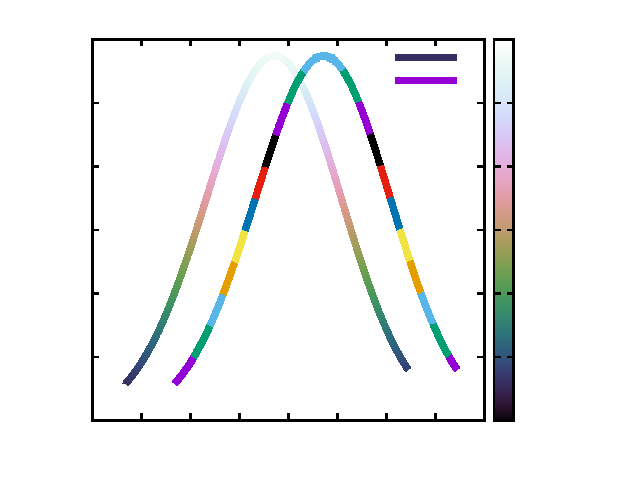
\includegraphics{figures/palette/plot}}%
    \gplfronttext
  \end{picture}%
\endgroup
}
    % }
\end{center}

\only<2>{\small See \url{http://colorbrewer2.org} for more colour series}
\end{frame}

\begin{frame}{Using}
    \begin{itemize}
        \item Select columns from data, e.g. \texttt{using 2:3} will use the second and third columns
        \item Special 0-th column with the number of point
        \item By enclosing it in \texttt{()}, you can operate on the numbers
        \begin{sitemize}
            \item \texttt{(1)} is a literal $1$
            \item \texttt{(\$1)} is the value of the first column
            \item \texttt{(\$2-\$1)} is the value of the second column minus the value of the first column
        \end{sitemize}
        \item You can have multiple dataset in the same file by splitting them with two newlines
        \begin{sitemize}
            \item \texttt{using 1:2 index 0} will select the first block
        \end{sitemize}
        \item There is also an \texttt{every i\_p:i\_b:s\_p:s\_b:e\_p:e\_b} directive 
        \begin{sitemize}
            \item \texttt{i}ncrement, \texttt{s}tart and \texttt{e}nd for \texttt{p}oints and \texttt{b}locks
        \end{sitemize}
    \end{itemize}
\end{frame}

\begin{frame}{Other plot types}
    \begin{itemize}
        \item \texttt{candlesticks} (box and whisker), that require 5 columns
        \item \texttt{boxes}, that act like impulse but with width and can be filled with solid or transparent colors or patterns
        \item \texttt{image}, that generate imagemaps (e.g. heatmaps)
        \item \texttt{label}, that writes the third column as a label at the coordinate defined by the first and second columns
        \item First column/row can be ignored by adding \texttt{rowheaders}/\texttt{columnheaders}
    \end{itemize}
\end{frame}

\begin{frame}{Stats}
    \begin{itemize}
        \item \texttt{stats 'file' \{using\} \{name 'p'\}} can be used to get statistics from files
        \item Same \texttt{using} options as \textit{plot}, but can only process up to 2 columns
        \item Several variables in the form \texttt{p\_variable} are assigned
        \begin{sitemize}
            \item \texttt{p} is the value of the \texttt{name} option, \texttt{STATS} if unset
            \item \texttt{\_x} and \texttt{\_y} suffixes if using 2 columns
        \end{sitemize}
        \item File variables
        \begin{sitemize}
            \item \texttt{records}, \texttt{blocks}, \texttt{columns} (of the first line!)
        \end{sitemize}
        \item 1-column variables
        \begin{sitemize}
            \item \texttt{min}, \texttt{max}, \texttt{mean}, \texttt{median}, \texttt{stdev}...
        \end{sitemize}
        \item 2-column variables
        \begin{sitemize}
            \item \texttt{correlation}, \texttt{slope}/\texttt{intercept} (linear fit)...
        \end{sitemize}
    \end{itemize}
\end{frame}

\begin{frame}{Table}
    \begin{itemize}
        \item \texttt{set table 'file'} 
        \item Will \textit{plot} to a file with a maximum of points defined by \texttt{set samples} in the  \texttt{x y\{ z\} r} format
        \begin{sitemize}
            \item \texttt{r} is either \texttt{i}n-range, \texttt{o}ut-of-range or \texttt{u}ndefined
        \end{sitemize}
        \item You can then \texttt{plot 'file'} to draw the plot
        \item Useful for reusing data or modifying it, e.g.
        \begin{sitemize}
            \item The values of a binning/smoothing
            \item The output of a function
        \end{sitemize}
        \item The table will have as many blocks as plots, e.g. \texttt{plot x, x**2} will generate a file with 2 blocks
    \end{itemize}
\end{frame}

\begin{frame}{Multiple axes}
    \begin{itemize}
        \item Every plot has two x and y axes
        \item \texttt{x2label}, \texttt{x2tics}, \texttt{x2range}
        \item \texttt{plot 'file' axes x1y2}
        \item Set \texttt{nomirror} for all tics
        \item \texttt{set link x2 via x**2 inverse sqrt(x)}
    \end{itemize}
\end{frame}

\begin{frame}{Multiple plots}
    \begin{itemize}
        \item \texttt{set multiplot} can be used to print multiple plots in the same \textit{page}
        \item \texttt{set multiplot layout 2,3 \{margins ...\}} for automatic overlay
        \begin{sitemize}
            \item \texttt{set multiplot next} can be used to skip one of the predefined spots
        \end{sitemize}
        \item \texttt{set origin x,y; set size x,y} for manual overlay of each plot
        \begin{sitemize}
            \item \texttt{0,0} is the bottom-left corner 
        \end{sitemize}
    \end{itemize}
\end{frame}

\begin{frame}{Key (legend)}
    \begin{itemize}
        \item Plots with empty title are not shown in the key
        \item \texttt{set key vertical maxrow 1} for horizontal key
        \item The key can be set at a relative position (inside/outside, top/bottom/left/right/center/etc.) or absolute (at 0.2, 0.3)
        \begin{sitemize}
            \item The coordinates are \textbf{x and y coordinates in the plot} by default!
            \item You can choose relative position in the graph (\texttt{at graph 0,0}) or whole image (\texttt{at screen 0,0}), with \texttt{0,0} = bottom left corner
        \end{sitemize}
    \end{itemize}
\end{frame}

\begin{frame}{Terminals}
    \begin{itemize}
        \item gnuplot has several \texttt{terminals} available
        \item Default terminal is the interactive \texttt{qt} or \texttt{x11} (depending on system defaults)
        \item Notable terminals are
        \begin{sitemize}
            % \item[\texttt{dumb}] outputs ASCII
            \item[\texttt{pngcairo}] outputs \texttt{.png}
            \item[\texttt{epslatex}] outputs a \texttt{.tex} and a \texttt{.eps} file, \texttt{input} the \texttt{.tex} file for inserting the image, will automatically inherit fonts!
            % \item[\texttt{epscairo}] for self-contained \texttt{.eps}
            \item[\texttt{svg}] for \texttt{.svg}
            \item[\texttt{canvas}] for partially interactive \texttt{html5} canvas objects
        \end{sitemize}
        \item Many behaviour differences between terminals
        \item Multiple parameters can be configured, depending on the terminal, e.g. mono/color, size, base linewidth, etc.
        \begin{sitemize}
            \item \texttt{enhanced} means \textit{enhanced} text, e.g. \texttt{a\_b} becomes a subscript. Will mess up your \LaTeX!
        \end{sitemize}
    \end{itemize}
\end{frame}

\begin{frame}[fragile]{Test}
\begin{center}
    % \resizebox{\linewidth}{!}{
        % GNUPLOT: LaTeX picture with Postscript
\begingroup
  \makeatletter
  \providecommand\color[2][]{%
    \GenericError{(gnuplot) \space\space\space\@spaces}{%
      Package color not loaded in conjunction with
      terminal option `colourtext'%
    }{See the gnuplot documentation for explanation.%
    }{Either use 'blacktext' in gnuplot or load the package
      color.sty in LaTeX.}%
    \renewcommand\color[2][]{}%
  }%
  \providecommand\includegraphics[2][]{%
    \GenericError{(gnuplot) \space\space\space\@spaces}{%
      Package graphicx or graphics not loaded%
    }{See the gnuplot documentation for explanation.%
    }{The gnuplot epslatex terminal needs graphicx.sty or graphics.sty.}%
    \renewcommand\includegraphics[2][]{}%
  }%
  \providecommand\rotatebox[2]{#2}%
  \@ifundefined{ifGPcolor}{%
    \newif\ifGPcolor
    \GPcolortrue
  }{}%
  \@ifundefined{ifGPblacktext}{%
    \newif\ifGPblacktext
    \GPblacktextfalse
  }{}%
  % define a \g@addto@macro without @ in the name:
  \let\gplgaddtomacro\g@addto@macro
  % define empty templates for all commands taking text:
  \gdef\gplbacktext{}%
  \gdef\gplfronttext{}%
  \makeatother
  \ifGPblacktext
    % no textcolor at all
    \def\colorrgb#1{}%
    \def\colorgray#1{}%
  \else
    % gray or color?
    \ifGPcolor
      \def\colorrgb#1{\color[rgb]{#1}}%
      \def\colorgray#1{\color[gray]{#1}}%
      \expandafter\def\csname LTw\endcsname{\color{white}}%
      \expandafter\def\csname LTb\endcsname{\color{black}}%
      \expandafter\def\csname LTa\endcsname{\color{black}}%
      \expandafter\def\csname LT0\endcsname{\color[rgb]{1,0,0}}%
      \expandafter\def\csname LT1\endcsname{\color[rgb]{0,1,0}}%
      \expandafter\def\csname LT2\endcsname{\color[rgb]{0,0,1}}%
      \expandafter\def\csname LT3\endcsname{\color[rgb]{1,0,1}}%
      \expandafter\def\csname LT4\endcsname{\color[rgb]{0,1,1}}%
      \expandafter\def\csname LT5\endcsname{\color[rgb]{1,1,0}}%
      \expandafter\def\csname LT6\endcsname{\color[rgb]{0,0,0}}%
      \expandafter\def\csname LT7\endcsname{\color[rgb]{1,0.3,0}}%
      \expandafter\def\csname LT8\endcsname{\color[rgb]{0.5,0.5,0.5}}%
    \else
      % gray
      \def\colorrgb#1{\color{black}}%
      \def\colorgray#1{\color[gray]{#1}}%
      \expandafter\def\csname LTw\endcsname{\color{white}}%
      \expandafter\def\csname LTb\endcsname{\color{black}}%
      \expandafter\def\csname LTa\endcsname{\color{black}}%
      \expandafter\def\csname LT0\endcsname{\color{black}}%
      \expandafter\def\csname LT1\endcsname{\color{black}}%
      \expandafter\def\csname LT2\endcsname{\color{black}}%
      \expandafter\def\csname LT3\endcsname{\color{black}}%
      \expandafter\def\csname LT4\endcsname{\color{black}}%
      \expandafter\def\csname LT5\endcsname{\color{black}}%
      \expandafter\def\csname LT6\endcsname{\color{black}}%
      \expandafter\def\csname LT7\endcsname{\color{black}}%
      \expandafter\def\csname LT8\endcsname{\color{black}}%
    \fi
  \fi
    \setlength{\unitlength}{0.0500bp}%
    \ifx\gptboxheight\undefined%
      \newlength{\gptboxheight}%
      \newlength{\gptboxwidth}%
      \newsavebox{\gptboxtext}%
    \fi%
    \setlength{\fboxrule}{0.5pt}%
    \setlength{\fboxsep}{1pt}%
\begin{picture}(5760.00,4320.00)%
    \gplgaddtomacro\gplfronttext{%
      \csname LTb\endcsname%%
      \put(264,4100){\makebox(0,0)[l]{\strut{}epslatex  terminal test}}%
      \put(264,3825){\makebox(0,0)[l]{\strut{}gnuplot version 5.2.2  }}%
      \csname LTb\endcsname%%
      \settowidth{\gptboxwidth}{\widthof{12345678901234567890}}
	\advance\gptboxwidth by 2\fboxsep
      \savebox{\gptboxtext}{\parbox[c][\totalheight+2\fboxsep]{\gptboxwidth}{\centering{12345678901234567890}}}
        \definecolor{tbcol}{rgb}{0.80,0.80,0.93}
	\put(2880,2160){\makebox[0.5\width][r]{\colorbox{tbcol}{\usebox{\gptboxtext}}}}
      \csname LTb\endcsname%%
      \put(2880,2490){\makebox(0,0){\strut{}true vs. estimated text dimensions}}%
      \put(2880,3480){\makebox(0,0)[l]{\strut{}left justified}}%
      \put(2880,3260){\makebox(0,0){\strut{}centre+d text}}%
      \put(2880,3040){\makebox(0,0)[r]{\strut{}right justified}}%
      \csname LT2\endcsname%%
      \put(2748,4100){\makebox(0,0)[r]{\strut{}show ticscale}}%
      \csname LTb\endcsname%%
      \put(4773,4100){\makebox(0,0)[r]{\strut{}-1}}%
      \csname LTa\endcsname%%
      \put(4773,3880){\makebox(0,0)[r]{\strut{}0}}%
      \colorrgb{0.58,0.00,0.83}%%
      \put(4773,3660){\makebox(0,0)[r]{\strut{}1}}%
      \colorrgb{0.00,0.62,0.45}%%
      \put(4773,3440){\makebox(0,0)[r]{\strut{}2}}%
      \colorrgb{0.34,0.71,0.91}%%
      \put(4773,3220){\makebox(0,0)[r]{\strut{}3}}%
      \colorrgb{0.90,0.62,0.00}%%
      \put(4773,3000){\makebox(0,0)[r]{\strut{}4}}%
      \colorrgb{0.94,0.89,0.26}%%
      \put(4773,2780){\makebox(0,0)[r]{\strut{}5}}%
      \colorrgb{0.00,0.45,0.70}%%
      \put(4773,2560){\makebox(0,0)[r]{\strut{}6}}%
      \colorrgb{0.90,0.12,0.06}%%
      \put(4773,2340){\makebox(0,0)[r]{\strut{}7}}%
      \colorrgb{0.00,0.00,0.00}%%
      \put(4773,2120){\makebox(0,0)[r]{\strut{}8}}%
      \colorrgb{0.58,0.00,0.83}%%
      \put(4773,1900){\makebox(0,0)[r]{\strut{}9}}%
      \colorrgb{0.00,0.62,0.45}%%
      \put(4773,1680){\makebox(0,0)[r]{\strut{}10}}%
      \colorrgb{0.34,0.71,0.91}%%
      \put(4773,1460){\makebox(0,0)[r]{\strut{}11}}%
      \colorrgb{0.90,0.62,0.00}%%
      \put(4773,1240){\makebox(0,0)[r]{\strut{}12}}%
      \colorrgb{0.94,0.89,0.26}%%
      \put(4773,1020){\makebox(0,0)[r]{\strut{}13}}%
      \colorrgb{0.00,0.45,0.70}%%
      \put(4773,800){\makebox(0,0)[r]{\strut{}14}}%
      \colorrgb{0.90,0.12,0.06}%%
      \put(4773,580){\makebox(0,0)[r]{\strut{}15}}%
      \colorrgb{0.00,0.00,0.00}%%
      \put(4773,360){\makebox(0,0)[r]{\strut{}16}}%
      \csname LT0\endcsname%%
      \put(220,2160){\rotatebox{-270}{\makebox(0,0){\strut{}rotated ce+ntred text}}}%
      \put(660,2160){\rotatebox{45}{\makebox(0,0)[l]{\strut{}  rotate by +45}}}%
      \put(660,2160){\rotatebox{-45}{\makebox(0,0)[l]{\strut{}  rotate by -45}}}%
      \csname LTb\endcsname%%
      \put(1008,172){\makebox(0,0)[l]{\strut{}  lw 1}}%
      \put(1008,344){\makebox(0,0)[l]{\strut{}  lw 2}}%
      \put(1008,516){\makebox(0,0)[l]{\strut{}  lw 3}}%
      \put(1008,688){\makebox(0,0)[l]{\strut{}  lw 4}}%
      \put(1008,860){\makebox(0,0)[l]{\strut{}  lw 5}}%
      \put(1008,1032){\makebox(0,0)[l]{\strut{}  lw 6}}%
      \put(432,1204){\makebox(0,0)[l]{\strut{}linewidth}}%
      \put(2304,172){\makebox(0,0)[l]{\strut{}  dt 1}}%
      \put(2304,344){\makebox(0,0)[l]{\strut{}  dt 2}}%
      \put(2304,516){\makebox(0,0)[l]{\strut{}  dt 3}}%
      \put(2304,688){\makebox(0,0)[l]{\strut{}  dt 4}}%
      \put(2304,860){\makebox(0,0)[l]{\strut{}  dt 5}}%
      \put(1728,1032){\makebox(0,0)[l]{\strut{}dashtype}}%
      \put(3888,870){\makebox(0,0){\strut{}pattern fill}}%
      \put(2952,650){\makebox(0,0){\strut{} 0}}%
      \put(3168,650){\makebox(0,0){\strut{} 1}}%
      \put(3384,650){\makebox(0,0){\strut{} 2}}%
      \put(3600,650){\makebox(0,0){\strut{} 3}}%
      \put(3816,650){\makebox(0,0){\strut{} 4}}%
      \put(4032,650){\makebox(0,0){\strut{} 5}}%
      \put(4248,650){\makebox(0,0){\strut{} 6}}%
      \put(4464,650){\makebox(0,0){\strut{} 7}}%
      \put(4680,650){\makebox(0,0){\strut{} 8}}%
      \csname LTb\endcsname%%
      \put(4031,3983){\makebox(0,0){\strut{}filled polygons:}}%
    }%
    \gplbacktext
    \put(0,0){\includegraphics{figures/test/plot}}%
    \gplfronttext
  \end{picture}%
\endgroup

    % }
\end{center}
\end{frame}

\begin{frame}[fragile]{Test with \texttt{dumb} terminal}
\tiny
\begin{verbatim}
gnuplot> set terminal test
Terminal type is now 'dumb'
Options are 'feed  size 79, 24 aspect 2, 1 mono'
gnuplot> test

+-dumb  terminal test-----------------show ticscale------------------1-+---+--+
|                                      $$$     filled polygons:      0 +...+ .|
| gnuplot version 5.2.2                :             XXXX            1 ***** A|
|                                      :             XXXXXXX         2 ##### B|
| ^            .>                      :            XXXXXXXXX        3 $$$$$ C|
| |          ..                        left justifieXXXXXXXXXX       4 %%%%% D|
| |        ..                    centre+d text       XXXXXXXX        5 @@@@@ E|
| |      ..             right justified:                XXXX         6 &&&&& F|
| |    ..                              :                             7 ===== G|
| |  ..                                :                             8 ***** H|
| |..                 true vs. estimated text dimensions             9 ***** I|
+.cannot rotate text.........+-------------------+..................10.#####.J+
| |  ..                                :                            11 $$$$$ K|
| |    ..                              :                 n+1        12 %%%%% L|
| |      ..                            Enhanced text:   x0          13 @@@@@ M|
| |        ..                          :               Bold Italic  14 &&&&& N|
| |          ..                        :                            15 ===== O|
| |            .                       :                            16 ***** P|
| |             >                      :                            17 ***** Q|
|                                      :      pattern fill          18 ##### R|
|                                               8                   19 $$$$$ S|
|                                      ||||||||||                   20 %%%%% T|
|                                      ||||||||||                             |
+----linewidthlw 6-----dashtype dt 5---++++++++++-----------------------------+

\end{verbatim}
    
\end{frame}

\begin{frame}{Coding}
\begin{itemize}
    \item Variables \texttt{x=2}
    \item Functions \texttt{max(x, y) = (x > y ? x : y)}
    \item Conditional \texttt{if (condition) something; else other thing;}
    \item Loops
    \begin{itemize}
        \item \texttt{do for [i=1:10] \{\dots\}}
        \item \texttt{plot for [i=1:10] \dots}
    \end{itemize}
    \item Simple string manipulation 
    \begin{sitemize}
        \item \texttt{a.'.txt'} concatenates
        \item \texttt{words("a b c") = 3}
        \item \texttt{word("a b c", 2) = b} (1-indexed)
    \end{sitemize}
    \item \texttt{system("ls")} for system calls
\end{itemize}
\end{frame}

\subsection{Recipes}

\begin{frame}{When to use \dots{}}
\begin{description}
    \item [\texttt{points}] for x/y plots, e.g. price of car vs max speed
    \begin{sitemize}
        \item Throw some fitted curves in (if it makes sense)
    \end{sitemize}
    \item [\texttt{lp}] for data with trends, e.g. speed vs fuel use
    \begin{sitemize}
        \item Only lines makes it very hard to read in b/w
        \item By using points on a subset of points you improve the readability
        \item Even better: manually set labels near points
    \end{sitemize}
    \item [\texttt{bars}]: for clustered data (e.g. histograms) or one axis is nominal e.g. car sales by brand
    \begin{sitemize}
        \item Can be rotated 90\textdegree{} to improve readability 
    \end{sitemize}
    \item [\texttt{box\&whisker}]: distribution of data, e.g. profit per car by year
    \begin{sitemize}
        \item Hides nonnormal distributions
        \item Better when supported with a violin plot!
    \end{sitemize}
\end{description}
\end{frame}

\begin{frame}{When to use \dots{} II}
\begin{description}
    \item [\texttt{heatmap}]: 3d data in 2d, e.g. confusion matrix
    \begin{sitemize}
        \item Hard to read unless data is sparse
    \end{sitemize}
    \item [\texttt{stacked}]: like lines but
    \begin{sitemize}
        \item Less intra-series resolution
        \item Easier to compare inter-series 
    \end{sitemize}
    \item [\texttt{circle}]: special kind of \texttt{point} where the third column defines the size of the point, e.g. bubble charts
    \item [\texttt{pie charts}]: no
    \item [\texttt{table}]: sometimes a plot is not the best way
    \begin{sitemize}
        \item All plots trade resolution for readability
        \item If you want $100\%$ precise readings, use a table
        \item Wrongly adding a table to your presentation is a nice way of losing the audience
    \end{sitemize}
\end{description}
\end{frame}


\begin{frame}{Box and violin plots}
\begin{center}
    % \resizebox{\linewidth}{!}{
        % GNUPLOT: LaTeX picture with Postscript
\begingroup
  \makeatletter
  \providecommand\color[2][]{%
    \GenericError{(gnuplot) \space\space\space\@spaces}{%
      Package color not loaded in conjunction with
      terminal option `colourtext'%
    }{See the gnuplot documentation for explanation.%
    }{Either use 'blacktext' in gnuplot or load the package
      color.sty in LaTeX.}%
    \renewcommand\color[2][]{}%
  }%
  \providecommand\includegraphics[2][]{%
    \GenericError{(gnuplot) \space\space\space\@spaces}{%
      Package graphicx or graphics not loaded%
    }{See the gnuplot documentation for explanation.%
    }{The gnuplot epslatex terminal needs graphicx.sty or graphics.sty.}%
    \renewcommand\includegraphics[2][]{}%
  }%
  \providecommand\rotatebox[2]{#2}%
  \@ifundefined{ifGPcolor}{%
    \newif\ifGPcolor
    \GPcolortrue
  }{}%
  \@ifundefined{ifGPblacktext}{%
    \newif\ifGPblacktext
    \GPblacktextfalse
  }{}%
  % define a \g@addto@macro without @ in the name:
  \let\gplgaddtomacro\g@addto@macro
  % define empty templates for all commands taking text:
  \gdef\gplbacktext{}%
  \gdef\gplfronttext{}%
  \makeatother
  \ifGPblacktext
    % no textcolor at all
    \def\colorrgb#1{}%
    \def\colorgray#1{}%
  \else
    % gray or color?
    \ifGPcolor
      \def\colorrgb#1{\color[rgb]{#1}}%
      \def\colorgray#1{\color[gray]{#1}}%
      \expandafter\def\csname LTw\endcsname{\color{white}}%
      \expandafter\def\csname LTb\endcsname{\color{black}}%
      \expandafter\def\csname LTa\endcsname{\color{black}}%
      \expandafter\def\csname LT0\endcsname{\color[rgb]{1,0,0}}%
      \expandafter\def\csname LT1\endcsname{\color[rgb]{0,1,0}}%
      \expandafter\def\csname LT2\endcsname{\color[rgb]{0,0,1}}%
      \expandafter\def\csname LT3\endcsname{\color[rgb]{1,0,1}}%
      \expandafter\def\csname LT4\endcsname{\color[rgb]{0,1,1}}%
      \expandafter\def\csname LT5\endcsname{\color[rgb]{1,1,0}}%
      \expandafter\def\csname LT6\endcsname{\color[rgb]{0,0,0}}%
      \expandafter\def\csname LT7\endcsname{\color[rgb]{1,0.3,0}}%
      \expandafter\def\csname LT8\endcsname{\color[rgb]{0.5,0.5,0.5}}%
    \else
      % gray
      \def\colorrgb#1{\color{black}}%
      \def\colorgray#1{\color[gray]{#1}}%
      \expandafter\def\csname LTw\endcsname{\color{white}}%
      \expandafter\def\csname LTb\endcsname{\color{black}}%
      \expandafter\def\csname LTa\endcsname{\color{black}}%
      \expandafter\def\csname LT0\endcsname{\color{black}}%
      \expandafter\def\csname LT1\endcsname{\color{black}}%
      \expandafter\def\csname LT2\endcsname{\color{black}}%
      \expandafter\def\csname LT3\endcsname{\color{black}}%
      \expandafter\def\csname LT4\endcsname{\color{black}}%
      \expandafter\def\csname LT5\endcsname{\color{black}}%
      \expandafter\def\csname LT6\endcsname{\color{black}}%
      \expandafter\def\csname LT7\endcsname{\color{black}}%
      \expandafter\def\csname LT8\endcsname{\color{black}}%
    \fi
  \fi
    \setlength{\unitlength}{0.0500bp}%
    \ifx\gptboxheight\undefined%
      \newlength{\gptboxheight}%
      \newlength{\gptboxwidth}%
      \newsavebox{\gptboxtext}%
    \fi%
    \setlength{\fboxrule}{0.5pt}%
    \setlength{\fboxsep}{1pt}%
\begin{picture}(5760.00,4320.00)%
    \gplgaddtomacro\gplbacktext{%
      \csname LTb\endcsname%%
      \put(594,440){\makebox(0,0)[r]{\strut{}$0$}}%
      \put(594,1050){\makebox(0,0)[r]{\strut{}$50$}}%
      \put(594,1660){\makebox(0,0)[r]{\strut{}$100$}}%
      \put(594,2270){\makebox(0,0)[r]{\strut{}$150$}}%
      \put(594,2879){\makebox(0,0)[r]{\strut{}$200$}}%
      \put(594,3489){\makebox(0,0)[r]{\strut{}$250$}}%
      \put(594,4099){\makebox(0,0)[r]{\strut{}$300$}}%
      \put(726,220){\makebox(0,0){\strut{}$32$}}%
      \put(1197,220){\makebox(0,0){\strut{}$33$}}%
      \put(1667,220){\makebox(0,0){\strut{}$34$}}%
      \put(2138,220){\makebox(0,0){\strut{}$35$}}%
      \put(2608,220){\makebox(0,0){\strut{}$36$}}%
      \put(3079,220){\makebox(0,0){\strut{}$37$}}%
      \put(3549,220){\makebox(0,0){\strut{}$38$}}%
      \put(4020,220){\makebox(0,0){\strut{}$39$}}%
      \put(4490,220){\makebox(0,0){\strut{}$40$}}%
    }%
    \gplgaddtomacro\gplfronttext{%
      \csname LTb\endcsname%%
      \put(3503,3926){\makebox(0,0)[r]{\strut{}u 1:2:2 w lc palette}}%
      \csname LTb\endcsname%%
      \put(3503,3706){\makebox(0,0)[r]{\strut{}u 1:2:2 w lc variable}}%
      \csname LTb\endcsname%%
      \put(4904,440){\makebox(0,0)[l]{\strut{}$0$}}%
      \put(4904,1049){\makebox(0,0)[l]{\strut{}$50$}}%
      \put(4904,1659){\makebox(0,0)[l]{\strut{}$100$}}%
      \put(4904,2269){\makebox(0,0)[l]{\strut{}$150$}}%
      \put(4904,2879){\makebox(0,0)[l]{\strut{}$200$}}%
      \put(4904,3489){\makebox(0,0)[l]{\strut{}$250$}}%
      \put(4904,4099){\makebox(0,0)[l]{\strut{}$300$}}%
    }%
    \gplbacktext
    \put(0,0){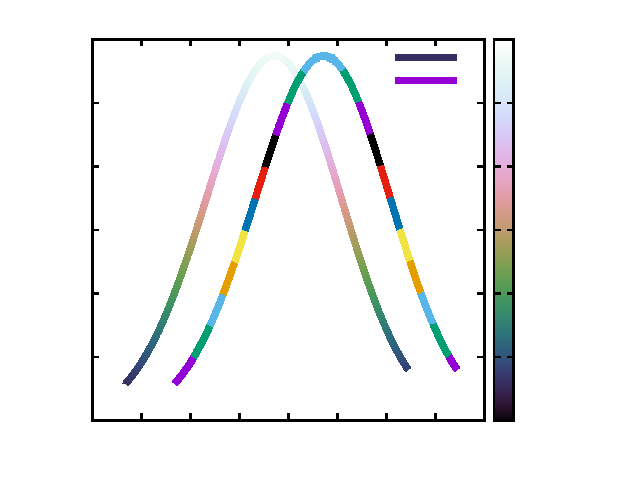
\includegraphics{figures/palette/plot}}%
    \gplfronttext
  \end{picture}%
\endgroup

    % }
\end{center}
\end{frame}

\begin{frame}[fragile]{Box and violin plots I}
\begin{verbatim}
set samples 3000
set boxwidth 0.25 absolute
set style fill solid 0.85 border lt -1
set style boxplot fraction 0.975 pt 6

bleuFiles=system("ls -1 stats/*Bleu.data")

unset xrange
do for [i=1:words(bleuFiles)] {
    set table 'bleu'.i
    plot word(bleuFiles,i) using 1 smooth kdensity \
    bandwidth 1
}
unset table
\end{verbatim}
\end{frame}

\begin{frame}[fragile]{Adjusting the number of tics}
\begin{verbatim}
mintics = 5

max(x, y) = (x > y ? x : y)
min(x, y) = (x < y ? x : y)
roundTo(x, y) = ceil(x/y)*y

maxV=0
minV=99999999
do for [i=1:words(bleuFiles)] {
    stats 'bleu'.i using 1 name 'y' nooutput;
    maxV=max(maxV, y_max);
    minV=min(minV, y_min);
}
set ytics roundTo((maxV-minV)/minTics, 1)
\end{verbatim}
\end{frame}

\begin{frame}[fragile]{Box and violin plots II}
\begin{verbatim}
tics=(0.5+words(bleuFiles))
set xrange [0.5:tics]

set ylabel "BLEU ($\rightarrow$)"
unset xtics
unset yrange
plot for [i=1:words(bleuFiles)] 'bleu'.i using \
        (i-$2/1000.):1 w lines ls (i) t '', \
    for [i=1:words(bleuFiles)] 'bleu'.i using \
        (i+$2/1000.):1 w lines ls (i) t '', \
    for [i=1:words(bleuFiles)] word(bleuFiles,i) \ 
        using (i):1 with boxplot fc ls i t ''

\end{verbatim}
\end{frame}

\begin{frame}{Heatmaps}
\begin{center}
    % \resizebox{0.7\linewidth}{!}{
        % GNUPLOT: LaTeX picture with Postscript
\begingroup
  \makeatletter
  \providecommand\color[2][]{%
    \GenericError{(gnuplot) \space\space\space\@spaces}{%
      Package color not loaded in conjunction with
      terminal option `colourtext'%
    }{See the gnuplot documentation for explanation.%
    }{Either use 'blacktext' in gnuplot or load the package
      color.sty in LaTeX.}%
    \renewcommand\color[2][]{}%
  }%
  \providecommand\includegraphics[2][]{%
    \GenericError{(gnuplot) \space\space\space\@spaces}{%
      Package graphicx or graphics not loaded%
    }{See the gnuplot documentation for explanation.%
    }{The gnuplot epslatex terminal needs graphicx.sty or graphics.sty.}%
    \renewcommand\includegraphics[2][]{}%
  }%
  \providecommand\rotatebox[2]{#2}%
  \@ifundefined{ifGPcolor}{%
    \newif\ifGPcolor
    \GPcolortrue
  }{}%
  \@ifundefined{ifGPblacktext}{%
    \newif\ifGPblacktext
    \GPblacktextfalse
  }{}%
  % define a \g@addto@macro without @ in the name:
  \let\gplgaddtomacro\g@addto@macro
  % define empty templates for all commands taking text:
  \gdef\gplbacktext{}%
  \gdef\gplfronttext{}%
  \makeatother
  \ifGPblacktext
    % no textcolor at all
    \def\colorrgb#1{}%
    \def\colorgray#1{}%
  \else
    % gray or color?
    \ifGPcolor
      \def\colorrgb#1{\color[rgb]{#1}}%
      \def\colorgray#1{\color[gray]{#1}}%
      \expandafter\def\csname LTw\endcsname{\color{white}}%
      \expandafter\def\csname LTb\endcsname{\color{black}}%
      \expandafter\def\csname LTa\endcsname{\color{black}}%
      \expandafter\def\csname LT0\endcsname{\color[rgb]{1,0,0}}%
      \expandafter\def\csname LT1\endcsname{\color[rgb]{0,1,0}}%
      \expandafter\def\csname LT2\endcsname{\color[rgb]{0,0,1}}%
      \expandafter\def\csname LT3\endcsname{\color[rgb]{1,0,1}}%
      \expandafter\def\csname LT4\endcsname{\color[rgb]{0,1,1}}%
      \expandafter\def\csname LT5\endcsname{\color[rgb]{1,1,0}}%
      \expandafter\def\csname LT6\endcsname{\color[rgb]{0,0,0}}%
      \expandafter\def\csname LT7\endcsname{\color[rgb]{1,0.3,0}}%
      \expandafter\def\csname LT8\endcsname{\color[rgb]{0.5,0.5,0.5}}%
    \else
      % gray
      \def\colorrgb#1{\color{black}}%
      \def\colorgray#1{\color[gray]{#1}}%
      \expandafter\def\csname LTw\endcsname{\color{white}}%
      \expandafter\def\csname LTb\endcsname{\color{black}}%
      \expandafter\def\csname LTa\endcsname{\color{black}}%
      \expandafter\def\csname LT0\endcsname{\color{black}}%
      \expandafter\def\csname LT1\endcsname{\color{black}}%
      \expandafter\def\csname LT2\endcsname{\color{black}}%
      \expandafter\def\csname LT3\endcsname{\color{black}}%
      \expandafter\def\csname LT4\endcsname{\color{black}}%
      \expandafter\def\csname LT5\endcsname{\color{black}}%
      \expandafter\def\csname LT6\endcsname{\color{black}}%
      \expandafter\def\csname LT7\endcsname{\color{black}}%
      \expandafter\def\csname LT8\endcsname{\color{black}}%
    \fi
  \fi
    \setlength{\unitlength}{0.0500bp}%
    \ifx\gptboxheight\undefined%
      \newlength{\gptboxheight}%
      \newlength{\gptboxwidth}%
      \newsavebox{\gptboxtext}%
    \fi%
    \setlength{\fboxrule}{0.5pt}%
    \setlength{\fboxsep}{1pt}%
\begin{picture}(5760.00,4320.00)%
    \gplgaddtomacro\gplbacktext{%
      \csname LTb\endcsname%%
      \put(594,440){\makebox(0,0)[r]{\strut{}$0$}}%
      \put(594,1050){\makebox(0,0)[r]{\strut{}$50$}}%
      \put(594,1660){\makebox(0,0)[r]{\strut{}$100$}}%
      \put(594,2270){\makebox(0,0)[r]{\strut{}$150$}}%
      \put(594,2879){\makebox(0,0)[r]{\strut{}$200$}}%
      \put(594,3489){\makebox(0,0)[r]{\strut{}$250$}}%
      \put(594,4099){\makebox(0,0)[r]{\strut{}$300$}}%
      \put(726,220){\makebox(0,0){\strut{}$32$}}%
      \put(1197,220){\makebox(0,0){\strut{}$33$}}%
      \put(1667,220){\makebox(0,0){\strut{}$34$}}%
      \put(2138,220){\makebox(0,0){\strut{}$35$}}%
      \put(2608,220){\makebox(0,0){\strut{}$36$}}%
      \put(3079,220){\makebox(0,0){\strut{}$37$}}%
      \put(3549,220){\makebox(0,0){\strut{}$38$}}%
      \put(4020,220){\makebox(0,0){\strut{}$39$}}%
      \put(4490,220){\makebox(0,0){\strut{}$40$}}%
    }%
    \gplgaddtomacro\gplfronttext{%
      \csname LTb\endcsname%%
      \put(3503,3926){\makebox(0,0)[r]{\strut{}u 1:2:2 w lc palette}}%
      \csname LTb\endcsname%%
      \put(3503,3706){\makebox(0,0)[r]{\strut{}u 1:2:2 w lc variable}}%
      \csname LTb\endcsname%%
      \put(4904,440){\makebox(0,0)[l]{\strut{}$0$}}%
      \put(4904,1049){\makebox(0,0)[l]{\strut{}$50$}}%
      \put(4904,1659){\makebox(0,0)[l]{\strut{}$100$}}%
      \put(4904,2269){\makebox(0,0)[l]{\strut{}$150$}}%
      \put(4904,2879){\makebox(0,0)[l]{\strut{}$200$}}%
      \put(4904,3489){\makebox(0,0)[l]{\strut{}$250$}}%
      \put(4904,4099){\makebox(0,0)[l]{\strut{}$300$}}%
    }%
    \gplbacktext
    \put(0,0){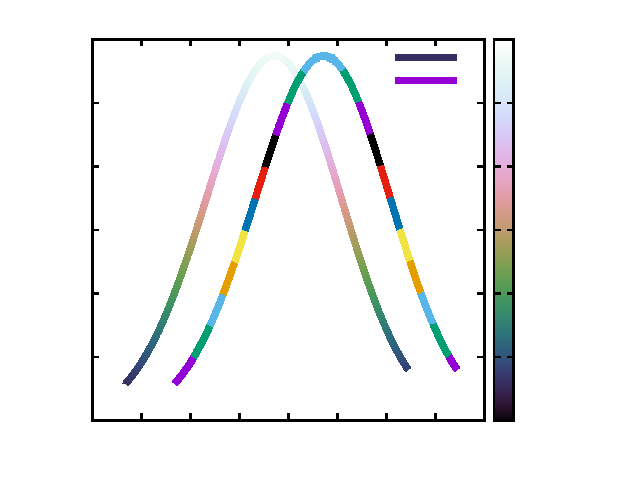
\includegraphics{figures/palette/plot}}%
    \gplfronttext
  \end{picture}%
\endgroup

    % }
\end{center}
\end{frame}

\begin{frame}[fragile]{Heatmaps I}
\begin{verbatim}
unset colorbox
set cbrange [-1:15]
set palette maxcolors 17
set palette model RGB defined (-1 '#FFFFFF', 
  0 '#1B9E77', 1 '#D95F02', 2 '#7570B3', 
  3 '#E7298A', 4 '#66A61E', 5 '#E6AB02', 
  6 '#A6761D', 7 '#F0027F', 8 '#8DD3C7', 
  9 '#BEBADA', 10 '#FB8072', 11 '#80B1D3', 
  12 '#FDB462', 13 '#B3DE69', 14 '#FCCDE5', 
  15 '#FF5555')

\end{verbatim}
\end{frame}

\begin{frame}[fragile]{Heatmaps II}
\begin{verbatim}
set grid front linetype -1 lw 1
set xtics scale 0 ("" 0.5)
set ytics scale 0 ("" 0.5)
set yrange [*:*] reverse
plot 'Bleu.significance' matrix with image t ''
\end{verbatim}
\end{frame}

\begin{frame}{Horizontal bars}
\begin{center}
    % \resizebox{\linewidth}{!}{
        % GNUPLOT: LaTeX picture with Postscript
\begingroup
  \makeatletter
  \providecommand\color[2][]{%
    \GenericError{(gnuplot) \space\space\space\@spaces}{%
      Package color not loaded in conjunction with
      terminal option `colourtext'%
    }{See the gnuplot documentation for explanation.%
    }{Either use 'blacktext' in gnuplot or load the package
      color.sty in LaTeX.}%
    \renewcommand\color[2][]{}%
  }%
  \providecommand\includegraphics[2][]{%
    \GenericError{(gnuplot) \space\space\space\@spaces}{%
      Package graphicx or graphics not loaded%
    }{See the gnuplot documentation for explanation.%
    }{The gnuplot epslatex terminal needs graphicx.sty or graphics.sty.}%
    \renewcommand\includegraphics[2][]{}%
  }%
  \providecommand\rotatebox[2]{#2}%
  \@ifundefined{ifGPcolor}{%
    \newif\ifGPcolor
    \GPcolortrue
  }{}%
  \@ifundefined{ifGPblacktext}{%
    \newif\ifGPblacktext
    \GPblacktextfalse
  }{}%
  % define a \g@addto@macro without @ in the name:
  \let\gplgaddtomacro\g@addto@macro
  % define empty templates for all commands taking text:
  \gdef\gplbacktext{}%
  \gdef\gplfronttext{}%
  \makeatother
  \ifGPblacktext
    % no textcolor at all
    \def\colorrgb#1{}%
    \def\colorgray#1{}%
  \else
    % gray or color?
    \ifGPcolor
      \def\colorrgb#1{\color[rgb]{#1}}%
      \def\colorgray#1{\color[gray]{#1}}%
      \expandafter\def\csname LTw\endcsname{\color{white}}%
      \expandafter\def\csname LTb\endcsname{\color{black}}%
      \expandafter\def\csname LTa\endcsname{\color{black}}%
      \expandafter\def\csname LT0\endcsname{\color[rgb]{1,0,0}}%
      \expandafter\def\csname LT1\endcsname{\color[rgb]{0,1,0}}%
      \expandafter\def\csname LT2\endcsname{\color[rgb]{0,0,1}}%
      \expandafter\def\csname LT3\endcsname{\color[rgb]{1,0,1}}%
      \expandafter\def\csname LT4\endcsname{\color[rgb]{0,1,1}}%
      \expandafter\def\csname LT5\endcsname{\color[rgb]{1,1,0}}%
      \expandafter\def\csname LT6\endcsname{\color[rgb]{0,0,0}}%
      \expandafter\def\csname LT7\endcsname{\color[rgb]{1,0.3,0}}%
      \expandafter\def\csname LT8\endcsname{\color[rgb]{0.5,0.5,0.5}}%
    \else
      % gray
      \def\colorrgb#1{\color{black}}%
      \def\colorgray#1{\color[gray]{#1}}%
      \expandafter\def\csname LTw\endcsname{\color{white}}%
      \expandafter\def\csname LTb\endcsname{\color{black}}%
      \expandafter\def\csname LTa\endcsname{\color{black}}%
      \expandafter\def\csname LT0\endcsname{\color{black}}%
      \expandafter\def\csname LT1\endcsname{\color{black}}%
      \expandafter\def\csname LT2\endcsname{\color{black}}%
      \expandafter\def\csname LT3\endcsname{\color{black}}%
      \expandafter\def\csname LT4\endcsname{\color{black}}%
      \expandafter\def\csname LT5\endcsname{\color{black}}%
      \expandafter\def\csname LT6\endcsname{\color{black}}%
      \expandafter\def\csname LT7\endcsname{\color{black}}%
      \expandafter\def\csname LT8\endcsname{\color{black}}%
    \fi
  \fi
    \setlength{\unitlength}{0.0500bp}%
    \ifx\gptboxheight\undefined%
      \newlength{\gptboxheight}%
      \newlength{\gptboxwidth}%
      \newsavebox{\gptboxtext}%
    \fi%
    \setlength{\fboxrule}{0.5pt}%
    \setlength{\fboxsep}{1pt}%
\begin{picture}(5760.00,4320.00)%
    \gplgaddtomacro\gplbacktext{%
      \csname LTb\endcsname%%
      \put(594,440){\makebox(0,0)[r]{\strut{}$0$}}%
      \put(594,1050){\makebox(0,0)[r]{\strut{}$50$}}%
      \put(594,1660){\makebox(0,0)[r]{\strut{}$100$}}%
      \put(594,2270){\makebox(0,0)[r]{\strut{}$150$}}%
      \put(594,2879){\makebox(0,0)[r]{\strut{}$200$}}%
      \put(594,3489){\makebox(0,0)[r]{\strut{}$250$}}%
      \put(594,4099){\makebox(0,0)[r]{\strut{}$300$}}%
      \put(726,220){\makebox(0,0){\strut{}$32$}}%
      \put(1197,220){\makebox(0,0){\strut{}$33$}}%
      \put(1667,220){\makebox(0,0){\strut{}$34$}}%
      \put(2138,220){\makebox(0,0){\strut{}$35$}}%
      \put(2608,220){\makebox(0,0){\strut{}$36$}}%
      \put(3079,220){\makebox(0,0){\strut{}$37$}}%
      \put(3549,220){\makebox(0,0){\strut{}$38$}}%
      \put(4020,220){\makebox(0,0){\strut{}$39$}}%
      \put(4490,220){\makebox(0,0){\strut{}$40$}}%
    }%
    \gplgaddtomacro\gplfronttext{%
      \csname LTb\endcsname%%
      \put(3503,3926){\makebox(0,0)[r]{\strut{}u 1:2:2 w lc palette}}%
      \csname LTb\endcsname%%
      \put(3503,3706){\makebox(0,0)[r]{\strut{}u 1:2:2 w lc variable}}%
      \csname LTb\endcsname%%
      \put(4904,440){\makebox(0,0)[l]{\strut{}$0$}}%
      \put(4904,1049){\makebox(0,0)[l]{\strut{}$50$}}%
      \put(4904,1659){\makebox(0,0)[l]{\strut{}$100$}}%
      \put(4904,2269){\makebox(0,0)[l]{\strut{}$150$}}%
      \put(4904,2879){\makebox(0,0)[l]{\strut{}$200$}}%
      \put(4904,3489){\makebox(0,0)[l]{\strut{}$250$}}%
      \put(4904,4099){\makebox(0,0)[l]{\strut{}$300$}}%
    }%
    \gplbacktext
    \put(0,0){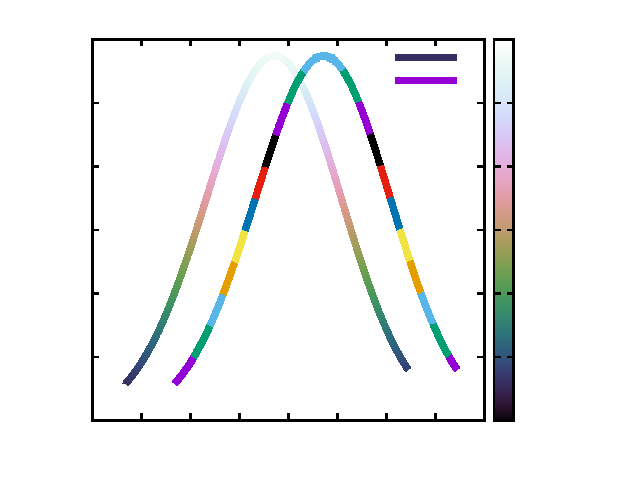
\includegraphics{figures/palette/plot}}%
    \gplfronttext
  \end{picture}%
\endgroup

    % }
\end{center}
\end{frame}

\begin{frame}[fragile]{Horizontal bars I}
\begin{verbatim}
set xrange[0:*]
set yrange[*:*] reverse
set title 'Entries per domain'
set xlabel '# of translations'
set ylabel ''
plot 'dom_count' u (0):($0):(0):2:($0-.5):($0+.5):ytic(1) \ 
  w boxxyerr ls 2 t ''

\end{verbatim}
\end{frame}

\begin{frame}{Subset}
\begin{center}
    % \resizebox{\linewidth}{!}{
        % GNUPLOT: LaTeX picture with Postscript
\begingroup
  \makeatletter
  \providecommand\color[2][]{%
    \GenericError{(gnuplot) \space\space\space\@spaces}{%
      Package color not loaded in conjunction with
      terminal option `colourtext'%
    }{See the gnuplot documentation for explanation.%
    }{Either use 'blacktext' in gnuplot or load the package
      color.sty in LaTeX.}%
    \renewcommand\color[2][]{}%
  }%
  \providecommand\includegraphics[2][]{%
    \GenericError{(gnuplot) \space\space\space\@spaces}{%
      Package graphicx or graphics not loaded%
    }{See the gnuplot documentation for explanation.%
    }{The gnuplot epslatex terminal needs graphicx.sty or graphics.sty.}%
    \renewcommand\includegraphics[2][]{}%
  }%
  \providecommand\rotatebox[2]{#2}%
  \@ifundefined{ifGPcolor}{%
    \newif\ifGPcolor
    \GPcolortrue
  }{}%
  \@ifundefined{ifGPblacktext}{%
    \newif\ifGPblacktext
    \GPblacktextfalse
  }{}%
  % define a \g@addto@macro without @ in the name:
  \let\gplgaddtomacro\g@addto@macro
  % define empty templates for all commands taking text:
  \gdef\gplbacktext{}%
  \gdef\gplfronttext{}%
  \makeatother
  \ifGPblacktext
    % no textcolor at all
    \def\colorrgb#1{}%
    \def\colorgray#1{}%
  \else
    % gray or color?
    \ifGPcolor
      \def\colorrgb#1{\color[rgb]{#1}}%
      \def\colorgray#1{\color[gray]{#1}}%
      \expandafter\def\csname LTw\endcsname{\color{white}}%
      \expandafter\def\csname LTb\endcsname{\color{black}}%
      \expandafter\def\csname LTa\endcsname{\color{black}}%
      \expandafter\def\csname LT0\endcsname{\color[rgb]{1,0,0}}%
      \expandafter\def\csname LT1\endcsname{\color[rgb]{0,1,0}}%
      \expandafter\def\csname LT2\endcsname{\color[rgb]{0,0,1}}%
      \expandafter\def\csname LT3\endcsname{\color[rgb]{1,0,1}}%
      \expandafter\def\csname LT4\endcsname{\color[rgb]{0,1,1}}%
      \expandafter\def\csname LT5\endcsname{\color[rgb]{1,1,0}}%
      \expandafter\def\csname LT6\endcsname{\color[rgb]{0,0,0}}%
      \expandafter\def\csname LT7\endcsname{\color[rgb]{1,0.3,0}}%
      \expandafter\def\csname LT8\endcsname{\color[rgb]{0.5,0.5,0.5}}%
    \else
      % gray
      \def\colorrgb#1{\color{black}}%
      \def\colorgray#1{\color[gray]{#1}}%
      \expandafter\def\csname LTw\endcsname{\color{white}}%
      \expandafter\def\csname LTb\endcsname{\color{black}}%
      \expandafter\def\csname LTa\endcsname{\color{black}}%
      \expandafter\def\csname LT0\endcsname{\color{black}}%
      \expandafter\def\csname LT1\endcsname{\color{black}}%
      \expandafter\def\csname LT2\endcsname{\color{black}}%
      \expandafter\def\csname LT3\endcsname{\color{black}}%
      \expandafter\def\csname LT4\endcsname{\color{black}}%
      \expandafter\def\csname LT5\endcsname{\color{black}}%
      \expandafter\def\csname LT6\endcsname{\color{black}}%
      \expandafter\def\csname LT7\endcsname{\color{black}}%
      \expandafter\def\csname LT8\endcsname{\color{black}}%
    \fi
  \fi
    \setlength{\unitlength}{0.0500bp}%
    \ifx\gptboxheight\undefined%
      \newlength{\gptboxheight}%
      \newlength{\gptboxwidth}%
      \newsavebox{\gptboxtext}%
    \fi%
    \setlength{\fboxrule}{0.5pt}%
    \setlength{\fboxsep}{1pt}%
\begin{picture}(5760.00,4320.00)%
    \gplgaddtomacro\gplbacktext{%
      \csname LTb\endcsname%%
      \put(594,440){\makebox(0,0)[r]{\strut{}$0$}}%
      \put(594,1050){\makebox(0,0)[r]{\strut{}$50$}}%
      \put(594,1660){\makebox(0,0)[r]{\strut{}$100$}}%
      \put(594,2270){\makebox(0,0)[r]{\strut{}$150$}}%
      \put(594,2879){\makebox(0,0)[r]{\strut{}$200$}}%
      \put(594,3489){\makebox(0,0)[r]{\strut{}$250$}}%
      \put(594,4099){\makebox(0,0)[r]{\strut{}$300$}}%
      \put(726,220){\makebox(0,0){\strut{}$32$}}%
      \put(1197,220){\makebox(0,0){\strut{}$33$}}%
      \put(1667,220){\makebox(0,0){\strut{}$34$}}%
      \put(2138,220){\makebox(0,0){\strut{}$35$}}%
      \put(2608,220){\makebox(0,0){\strut{}$36$}}%
      \put(3079,220){\makebox(0,0){\strut{}$37$}}%
      \put(3549,220){\makebox(0,0){\strut{}$38$}}%
      \put(4020,220){\makebox(0,0){\strut{}$39$}}%
      \put(4490,220){\makebox(0,0){\strut{}$40$}}%
    }%
    \gplgaddtomacro\gplfronttext{%
      \csname LTb\endcsname%%
      \put(3503,3926){\makebox(0,0)[r]{\strut{}u 1:2:2 w lc palette}}%
      \csname LTb\endcsname%%
      \put(3503,3706){\makebox(0,0)[r]{\strut{}u 1:2:2 w lc variable}}%
      \csname LTb\endcsname%%
      \put(4904,440){\makebox(0,0)[l]{\strut{}$0$}}%
      \put(4904,1049){\makebox(0,0)[l]{\strut{}$50$}}%
      \put(4904,1659){\makebox(0,0)[l]{\strut{}$100$}}%
      \put(4904,2269){\makebox(0,0)[l]{\strut{}$150$}}%
      \put(4904,2879){\makebox(0,0)[l]{\strut{}$200$}}%
      \put(4904,3489){\makebox(0,0)[l]{\strut{}$250$}}%
      \put(4904,4099){\makebox(0,0)[l]{\strut{}$300$}}%
    }%
    \gplbacktext
    \put(0,0){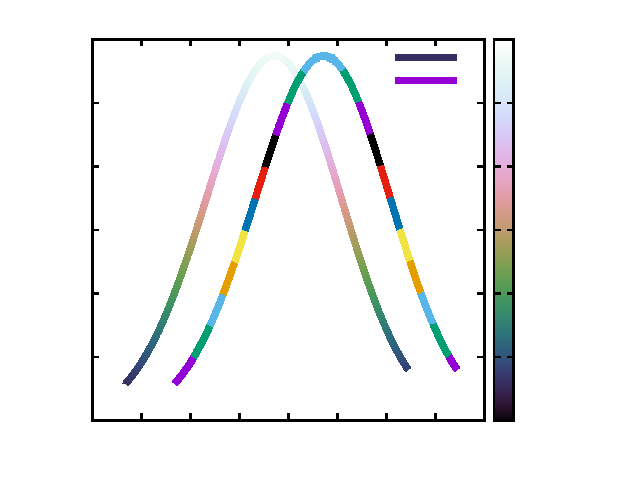
\includegraphics{figures/palette/plot}}%
    \gplfronttext
  \end{picture}%
\endgroup

    % }
\end{center}
\end{frame}

\begin{frame}{Multiplot}
\begin{center}
    % \resizebox{\linewidth}{!}{
        % GNUPLOT: LaTeX picture with Postscript
\begingroup
  \makeatletter
  \providecommand\color[2][]{%
    \GenericError{(gnuplot) \space\space\space\@spaces}{%
      Package color not loaded in conjunction with
      terminal option `colourtext'%
    }{See the gnuplot documentation for explanation.%
    }{Either use 'blacktext' in gnuplot or load the package
      color.sty in LaTeX.}%
    \renewcommand\color[2][]{}%
  }%
  \providecommand\includegraphics[2][]{%
    \GenericError{(gnuplot) \space\space\space\@spaces}{%
      Package graphicx or graphics not loaded%
    }{See the gnuplot documentation for explanation.%
    }{The gnuplot epslatex terminal needs graphicx.sty or graphics.sty.}%
    \renewcommand\includegraphics[2][]{}%
  }%
  \providecommand\rotatebox[2]{#2}%
  \@ifundefined{ifGPcolor}{%
    \newif\ifGPcolor
    \GPcolortrue
  }{}%
  \@ifundefined{ifGPblacktext}{%
    \newif\ifGPblacktext
    \GPblacktextfalse
  }{}%
  % define a \g@addto@macro without @ in the name:
  \let\gplgaddtomacro\g@addto@macro
  % define empty templates for all commands taking text:
  \gdef\gplbacktext{}%
  \gdef\gplfronttext{}%
  \makeatother
  \ifGPblacktext
    % no textcolor at all
    \def\colorrgb#1{}%
    \def\colorgray#1{}%
  \else
    % gray or color?
    \ifGPcolor
      \def\colorrgb#1{\color[rgb]{#1}}%
      \def\colorgray#1{\color[gray]{#1}}%
      \expandafter\def\csname LTw\endcsname{\color{white}}%
      \expandafter\def\csname LTb\endcsname{\color{black}}%
      \expandafter\def\csname LTa\endcsname{\color{black}}%
      \expandafter\def\csname LT0\endcsname{\color[rgb]{1,0,0}}%
      \expandafter\def\csname LT1\endcsname{\color[rgb]{0,1,0}}%
      \expandafter\def\csname LT2\endcsname{\color[rgb]{0,0,1}}%
      \expandafter\def\csname LT3\endcsname{\color[rgb]{1,0,1}}%
      \expandafter\def\csname LT4\endcsname{\color[rgb]{0,1,1}}%
      \expandafter\def\csname LT5\endcsname{\color[rgb]{1,1,0}}%
      \expandafter\def\csname LT6\endcsname{\color[rgb]{0,0,0}}%
      \expandafter\def\csname LT7\endcsname{\color[rgb]{1,0.3,0}}%
      \expandafter\def\csname LT8\endcsname{\color[rgb]{0.5,0.5,0.5}}%
    \else
      % gray
      \def\colorrgb#1{\color{black}}%
      \def\colorgray#1{\color[gray]{#1}}%
      \expandafter\def\csname LTw\endcsname{\color{white}}%
      \expandafter\def\csname LTb\endcsname{\color{black}}%
      \expandafter\def\csname LTa\endcsname{\color{black}}%
      \expandafter\def\csname LT0\endcsname{\color{black}}%
      \expandafter\def\csname LT1\endcsname{\color{black}}%
      \expandafter\def\csname LT2\endcsname{\color{black}}%
      \expandafter\def\csname LT3\endcsname{\color{black}}%
      \expandafter\def\csname LT4\endcsname{\color{black}}%
      \expandafter\def\csname LT5\endcsname{\color{black}}%
      \expandafter\def\csname LT6\endcsname{\color{black}}%
      \expandafter\def\csname LT7\endcsname{\color{black}}%
      \expandafter\def\csname LT8\endcsname{\color{black}}%
    \fi
  \fi
    \setlength{\unitlength}{0.0500bp}%
    \ifx\gptboxheight\undefined%
      \newlength{\gptboxheight}%
      \newlength{\gptboxwidth}%
      \newsavebox{\gptboxtext}%
    \fi%
    \setlength{\fboxrule}{0.5pt}%
    \setlength{\fboxsep}{1pt}%
\begin{picture}(5760.00,4320.00)%
    \gplgaddtomacro\gplbacktext{%
      \csname LTb\endcsname%%
      \put(594,3680){\makebox(0,0)[r]{\strut{}$-10$}}%
      \put(594,3785){\makebox(0,0)[r]{\strut{}$-5$}}%
      \put(594,3890){\makebox(0,0)[r]{\strut{}$0$}}%
      \put(594,3994){\makebox(0,0)[r]{\strut{}$5$}}%
      \put(594,4099){\makebox(0,0)[r]{\strut{}$10$}}%
      \put(726,3460){\makebox(0,0){\strut{}$-10$}}%
      \put(805,3460){\makebox(0,0){\strut{}$-5$}}%
      \put(885,3460){\makebox(0,0){\strut{}$0$}}%
      \put(964,3460){\makebox(0,0){\strut{}$5$}}%
      \put(1043,3460){\makebox(0,0){\strut{}$10$}}%
    }%
    \gplgaddtomacro\gplfronttext{%
      \csname LTb\endcsname%%
      \put(56,3926){\makebox(0,0)[r]{\strut{}x}}%
    }%
    \gplgaddtomacro\gplbacktext{%
      \csname LTb\endcsname%%
      \put(594,2600){\makebox(0,0)[r]{\strut{}$-10$}}%
      \put(594,2705){\makebox(0,0)[r]{\strut{}$-5$}}%
      \put(594,2810){\makebox(0,0)[r]{\strut{}$0$}}%
      \put(594,2914){\makebox(0,0)[r]{\strut{}$5$}}%
      \put(594,3019){\makebox(0,0)[r]{\strut{}$10$}}%
      \put(726,2380){\makebox(0,0){\strut{}$-10$}}%
      \put(805,2380){\makebox(0,0){\strut{}$-5$}}%
      \put(885,2380){\makebox(0,0){\strut{}$0$}}%
      \put(964,2380){\makebox(0,0){\strut{}$5$}}%
      \put(1043,2380){\makebox(0,0){\strut{}$10$}}%
    }%
    \gplgaddtomacro\gplfronttext{%
      \csname LTb\endcsname%%
      \put(56,2846){\makebox(0,0)[r]{\strut{}x}}%
    }%
    \gplgaddtomacro\gplfronttext{%
      \csname LTb\endcsname%%
      \put(1704,4100){\makebox(0,0)[l]{\strut{}epslatex  terminal test}}%
      \put(1704,3825){\makebox(0,0)[l]{\strut{}gnuplot version 5.2.2  }}%
      \csname LTb\endcsname%%
      \settowidth{\gptboxwidth}{\widthof{12345678901234567890}}
	\advance\gptboxwidth by 2\fboxsep
      \savebox{\gptboxtext}{\parbox[c][\totalheight+2\fboxsep]{\gptboxwidth}{\centering{12345678901234567890}}}
        \definecolor{tbcol}{rgb}{0.80,0.80,0.93}
	\put(2160,1620){\makebox[0.5\width][r]{\colorbox{tbcol}{\usebox{\gptboxtext}}}}
      \csname LTb\endcsname%%
      \put(2160,1950){\makebox(0,0){\strut{}true vs. estimated text dimensions}}%
      \put(3600,4020){\makebox(0,0)[l]{\strut{}left justified}}%
      \put(3600,3800){\makebox(0,0){\strut{}centre+d text}}%
      \put(3600,3580){\makebox(0,0)[r]{\strut{}right justified}}%
      \csname LT2\endcsname%%
      \put(3468,4100){\makebox(0,0)[r]{\strut{}show ticscale}}%
      \csname LTb\endcsname%%
      \put(4773,4100){\makebox(0,0)[r]{\strut{}-1}}%
      \csname LTa\endcsname%%
      \put(4773,3880){\makebox(0,0)[r]{\strut{}0}}%
      \colorrgb{0.58,0.00,0.83}%%
      \put(4773,3660){\makebox(0,0)[r]{\strut{}1}}%
      \colorrgb{0.00,0.62,0.45}%%
      \put(4773,3440){\makebox(0,0)[r]{\strut{}2}}%
      \colorrgb{0.34,0.71,0.91}%%
      \put(4773,3220){\makebox(0,0)[r]{\strut{}3}}%
      \colorrgb{0.90,0.62,0.00}%%
      \put(4773,3000){\makebox(0,0)[r]{\strut{}4}}%
      \colorrgb{0.94,0.89,0.26}%%
      \put(4773,2780){\makebox(0,0)[r]{\strut{}5}}%
      \colorrgb{0.00,0.45,0.70}%%
      \put(4773,2560){\makebox(0,0)[r]{\strut{}6}}%
      \colorrgb{0.90,0.12,0.06}%%
      \put(4773,2340){\makebox(0,0)[r]{\strut{}7}}%
      \colorrgb{0.00,0.00,0.00}%%
      \put(4773,2120){\makebox(0,0)[r]{\strut{}8}}%
      \colorrgb{0.58,0.00,0.83}%%
      \put(4773,1900){\makebox(0,0)[r]{\strut{}9}}%
      \colorrgb{0.00,0.62,0.45}%%
      \put(4773,1680){\makebox(0,0)[r]{\strut{}10}}%
      \colorrgb{0.34,0.71,0.91}%%
      \put(4773,1460){\makebox(0,0)[r]{\strut{}11}}%
      \csname LT0\endcsname%%
      \put(1660,2700){\rotatebox{-270}{\makebox(0,0){\strut{}rotated ce+ntred text}}}%
      \put(2100,2700){\rotatebox{45}{\makebox(0,0)[l]{\strut{}  rotate by +45}}}%
      \put(2100,2700){\rotatebox{-45}{\makebox(0,0)[l]{\strut{}  rotate by -45}}}%
      \csname LTb\endcsname%%
      \put(2196,1209){\makebox(0,0)[l]{\strut{}  lw 1}}%
      \put(2196,1338){\makebox(0,0)[l]{\strut{}  lw 2}}%
      \put(2196,1467){\makebox(0,0)[l]{\strut{}  lw 3}}%
      \put(2196,1596){\makebox(0,0)[l]{\strut{}  lw 4}}%
      \put(2196,1725){\makebox(0,0)[l]{\strut{}  lw 5}}%
      \put(2196,1854){\makebox(0,0)[l]{\strut{}  lw 6}}%
      \put(1764,1983){\makebox(0,0)[l]{\strut{}linewidth}}%
      \put(3168,1209){\makebox(0,0)[l]{\strut{}  dt 1}}%
      \put(3168,1338){\makebox(0,0)[l]{\strut{}  dt 2}}%
      \put(3168,1467){\makebox(0,0)[l]{\strut{}  dt 3}}%
      \put(3168,1596){\makebox(0,0)[l]{\strut{}  dt 4}}%
      \put(3168,1725){\makebox(0,0)[l]{\strut{}  dt 5}}%
      \put(2736,1854){\makebox(0,0)[l]{\strut{}dashtype}}%
      \put(4356,1815){\makebox(0,0){\strut{}pattern fill}}%
      \put(3654,1595){\makebox(0,0){\strut{} 0}}%
      \put(3816,1595){\makebox(0,0){\strut{} 1}}%
      \put(3978,1595){\makebox(0,0){\strut{} 2}}%
      \put(4140,1595){\makebox(0,0){\strut{} 3}}%
      \put(4302,1595){\makebox(0,0){\strut{} 4}}%
      \put(4464,1595){\makebox(0,0){\strut{} 5}}%
      \put(4626,1595){\makebox(0,0){\strut{} 6}}%
      \put(4788,1595){\makebox(0,0){\strut{} 7}}%
      \put(4950,1595){\makebox(0,0){\strut{} 8}}%
      \csname LTb\endcsname%%
      \put(4464,4095){\makebox(0,0){\strut{}filled polygons:}}%
    }%
    \gplgaddtomacro\gplbacktext{%
      \csname LTb\endcsname%%
      \put(462,440){\makebox(0,0)[r]{\strut{}$-2$}}%
      \put(462,628){\makebox(0,0)[r]{\strut{}$0$}}%
      \put(462,815){\makebox(0,0)[r]{\strut{}$2$}}%
      \put(462,1003){\makebox(0,0)[r]{\strut{}$4$}}%
      \put(462,1190){\makebox(0,0)[r]{\strut{}$6$}}%
      \put(462,1378){\makebox(0,0)[r]{\strut{}$8$}}%
      \put(462,1565){\makebox(0,0)[r]{\strut{}$10$}}%
      \put(462,1753){\makebox(0,0)[r]{\strut{}$12$}}%
      \put(462,1940){\makebox(0,0)[r]{\strut{}$14$}}%
      \put(594,220){\makebox(0,0){\strut{}$-2$}}%
      \put(755,220){\makebox(0,0){\strut{}$0$}}%
      \put(917,220){\makebox(0,0){\strut{}$2$}}%
      \put(1078,220){\makebox(0,0){\strut{}$4$}}%
      \put(1239,220){\makebox(0,0){\strut{}$6$}}%
      \put(1400,220){\makebox(0,0){\strut{}$8$}}%
      \put(1562,220){\makebox(0,0){\strut{}$10$}}%
      \put(1723,220){\makebox(0,0){\strut{}$12$}}%
      \put(1884,220){\makebox(0,0){\strut{}$14$}}%
    }%
    \gplgaddtomacro\gplfronttext{%
      \csname LTb\endcsname%%
      \put(2112,440){\makebox(0,0)[l]{\strut{}$-2$}}%
      \put(2112,654){\makebox(0,0)[l]{\strut{}$0$}}%
      \put(2112,868){\makebox(0,0)[l]{\strut{}$2$}}%
      \put(2112,1082){\makebox(0,0)[l]{\strut{}$4$}}%
      \put(2112,1297){\makebox(0,0)[l]{\strut{}$6$}}%
      \put(2112,1511){\makebox(0,0)[l]{\strut{}$8$}}%
      \put(2112,1725){\makebox(0,0)[l]{\strut{}$10$}}%
      \put(2112,1940){\makebox(0,0)[l]{\strut{}$12$}}%
    }%
    \gplgaddtomacro\gplbacktext{%
      \csname LTb\endcsname%%
      \put(3474,440){\makebox(0,0)[r]{\strut{}$0$}}%
      \put(3474,510){\makebox(0,0)[r]{\strut{}$50$}}%
      \put(3474,580){\makebox(0,0)[r]{\strut{}$100$}}%
      \put(3474,650){\makebox(0,0)[r]{\strut{}$150$}}%
      \put(3474,720){\makebox(0,0)[r]{\strut{}$200$}}%
      \put(3474,790){\makebox(0,0)[r]{\strut{}$250$}}%
      \put(3474,860){\makebox(0,0)[r]{\strut{}$300$}}%
      \put(3606,220){\makebox(0,0){\strut{}$32$}}%
      \put(3651,220){\makebox(0,0){\strut{}$33$}}%
      \put(3697,220){\makebox(0,0){\strut{}$34$}}%
      \put(3742,220){\makebox(0,0){\strut{}$35$}}%
      \put(3787,220){\makebox(0,0){\strut{}$36$}}%
      \put(3832,220){\makebox(0,0){\strut{}$37$}}%
      \put(3878,220){\makebox(0,0){\strut{}$38$}}%
      \put(3923,220){\makebox(0,0){\strut{}$39$}}%
    }%
    \gplgaddtomacro\gplfronttext{%
      \csname LTb\endcsname%%
      \put(2936,687){\makebox(0,0)[r]{\strut{}'bleu1'}}%
    }%
    \gplgaddtomacro\gplbacktext{%
      \csname LTb\endcsname%%
      \put(4914,440){\makebox(0,0)[r]{\strut{}$0$}}%
      \put(4914,510){\makebox(0,0)[r]{\strut{}$50$}}%
      \put(4914,580){\makebox(0,0)[r]{\strut{}$100$}}%
      \put(4914,650){\makebox(0,0)[r]{\strut{}$150$}}%
      \put(4914,720){\makebox(0,0)[r]{\strut{}$200$}}%
      \put(4914,790){\makebox(0,0)[r]{\strut{}$250$}}%
      \put(4914,860){\makebox(0,0)[r]{\strut{}$300$}}%
      \put(5046,220){\makebox(0,0){\strut{}$32$}}%
      \put(5091,220){\makebox(0,0){\strut{}$33$}}%
      \put(5137,220){\makebox(0,0){\strut{}$34$}}%
      \put(5182,220){\makebox(0,0){\strut{}$35$}}%
      \put(5227,220){\makebox(0,0){\strut{}$36$}}%
      \put(5272,220){\makebox(0,0){\strut{}$37$}}%
      \put(5318,220){\makebox(0,0){\strut{}$38$}}%
      \put(5363,220){\makebox(0,0){\strut{}$39$}}%
    }%
    \gplgaddtomacro\gplfronttext{%
      \csname LTb\endcsname%%
      \put(4376,687){\makebox(0,0)[r]{\strut{}'bleu2'}}%
    }%
    \gplbacktext
    \put(0,0){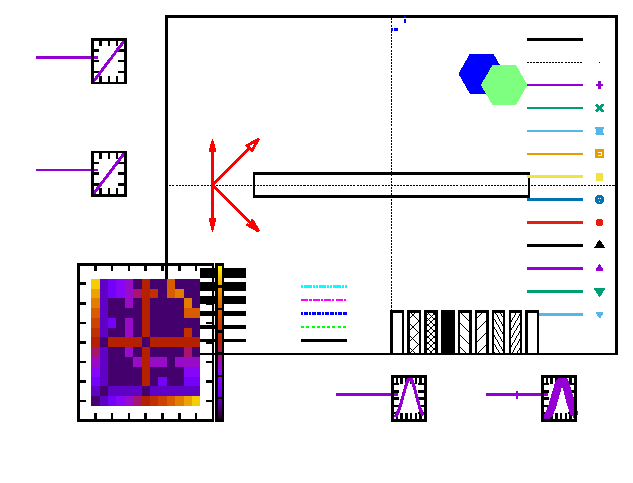
\includegraphics{figures/multiplot1/plot}}%
    \gplfronttext
  \end{picture}%
\endgroup

    % }
\end{center}
\end{frame}

\begin{frame}{Palette and variable}
\begin{center}
    % \resizebox{\linewidth}{!}{
        % GNUPLOT: LaTeX picture with Postscript
\begingroup
  \makeatletter
  \providecommand\color[2][]{%
    \GenericError{(gnuplot) \space\space\space\@spaces}{%
      Package color not loaded in conjunction with
      terminal option `colourtext'%
    }{See the gnuplot documentation for explanation.%
    }{Either use 'blacktext' in gnuplot or load the package
      color.sty in LaTeX.}%
    \renewcommand\color[2][]{}%
  }%
  \providecommand\includegraphics[2][]{%
    \GenericError{(gnuplot) \space\space\space\@spaces}{%
      Package graphicx or graphics not loaded%
    }{See the gnuplot documentation for explanation.%
    }{The gnuplot epslatex terminal needs graphicx.sty or graphics.sty.}%
    \renewcommand\includegraphics[2][]{}%
  }%
  \providecommand\rotatebox[2]{#2}%
  \@ifundefined{ifGPcolor}{%
    \newif\ifGPcolor
    \GPcolortrue
  }{}%
  \@ifundefined{ifGPblacktext}{%
    \newif\ifGPblacktext
    \GPblacktextfalse
  }{}%
  % define a \g@addto@macro without @ in the name:
  \let\gplgaddtomacro\g@addto@macro
  % define empty templates for all commands taking text:
  \gdef\gplbacktext{}%
  \gdef\gplfronttext{}%
  \makeatother
  \ifGPblacktext
    % no textcolor at all
    \def\colorrgb#1{}%
    \def\colorgray#1{}%
  \else
    % gray or color?
    \ifGPcolor
      \def\colorrgb#1{\color[rgb]{#1}}%
      \def\colorgray#1{\color[gray]{#1}}%
      \expandafter\def\csname LTw\endcsname{\color{white}}%
      \expandafter\def\csname LTb\endcsname{\color{black}}%
      \expandafter\def\csname LTa\endcsname{\color{black}}%
      \expandafter\def\csname LT0\endcsname{\color[rgb]{1,0,0}}%
      \expandafter\def\csname LT1\endcsname{\color[rgb]{0,1,0}}%
      \expandafter\def\csname LT2\endcsname{\color[rgb]{0,0,1}}%
      \expandafter\def\csname LT3\endcsname{\color[rgb]{1,0,1}}%
      \expandafter\def\csname LT4\endcsname{\color[rgb]{0,1,1}}%
      \expandafter\def\csname LT5\endcsname{\color[rgb]{1,1,0}}%
      \expandafter\def\csname LT6\endcsname{\color[rgb]{0,0,0}}%
      \expandafter\def\csname LT7\endcsname{\color[rgb]{1,0.3,0}}%
      \expandafter\def\csname LT8\endcsname{\color[rgb]{0.5,0.5,0.5}}%
    \else
      % gray
      \def\colorrgb#1{\color{black}}%
      \def\colorgray#1{\color[gray]{#1}}%
      \expandafter\def\csname LTw\endcsname{\color{white}}%
      \expandafter\def\csname LTb\endcsname{\color{black}}%
      \expandafter\def\csname LTa\endcsname{\color{black}}%
      \expandafter\def\csname LT0\endcsname{\color{black}}%
      \expandafter\def\csname LT1\endcsname{\color{black}}%
      \expandafter\def\csname LT2\endcsname{\color{black}}%
      \expandafter\def\csname LT3\endcsname{\color{black}}%
      \expandafter\def\csname LT4\endcsname{\color{black}}%
      \expandafter\def\csname LT5\endcsname{\color{black}}%
      \expandafter\def\csname LT6\endcsname{\color{black}}%
      \expandafter\def\csname LT7\endcsname{\color{black}}%
      \expandafter\def\csname LT8\endcsname{\color{black}}%
    \fi
  \fi
    \setlength{\unitlength}{0.0500bp}%
    \ifx\gptboxheight\undefined%
      \newlength{\gptboxheight}%
      \newlength{\gptboxwidth}%
      \newsavebox{\gptboxtext}%
    \fi%
    \setlength{\fboxrule}{0.5pt}%
    \setlength{\fboxsep}{1pt}%
\begin{picture}(5760.00,4320.00)%
    \gplgaddtomacro\gplbacktext{%
      \csname LTb\endcsname%%
      \put(594,440){\makebox(0,0)[r]{\strut{}$0$}}%
      \put(594,1050){\makebox(0,0)[r]{\strut{}$50$}}%
      \put(594,1660){\makebox(0,0)[r]{\strut{}$100$}}%
      \put(594,2270){\makebox(0,0)[r]{\strut{}$150$}}%
      \put(594,2879){\makebox(0,0)[r]{\strut{}$200$}}%
      \put(594,3489){\makebox(0,0)[r]{\strut{}$250$}}%
      \put(594,4099){\makebox(0,0)[r]{\strut{}$300$}}%
      \put(726,220){\makebox(0,0){\strut{}$32$}}%
      \put(1197,220){\makebox(0,0){\strut{}$33$}}%
      \put(1667,220){\makebox(0,0){\strut{}$34$}}%
      \put(2138,220){\makebox(0,0){\strut{}$35$}}%
      \put(2608,220){\makebox(0,0){\strut{}$36$}}%
      \put(3079,220){\makebox(0,0){\strut{}$37$}}%
      \put(3549,220){\makebox(0,0){\strut{}$38$}}%
      \put(4020,220){\makebox(0,0){\strut{}$39$}}%
      \put(4490,220){\makebox(0,0){\strut{}$40$}}%
    }%
    \gplgaddtomacro\gplfronttext{%
      \csname LTb\endcsname%%
      \put(3503,3926){\makebox(0,0)[r]{\strut{}u 1:2:2 w lc palette}}%
      \csname LTb\endcsname%%
      \put(3503,3706){\makebox(0,0)[r]{\strut{}u 1:2:2 w lc variable}}%
      \csname LTb\endcsname%%
      \put(4904,440){\makebox(0,0)[l]{\strut{}$0$}}%
      \put(4904,1049){\makebox(0,0)[l]{\strut{}$50$}}%
      \put(4904,1659){\makebox(0,0)[l]{\strut{}$100$}}%
      \put(4904,2269){\makebox(0,0)[l]{\strut{}$150$}}%
      \put(4904,2879){\makebox(0,0)[l]{\strut{}$200$}}%
      \put(4904,3489){\makebox(0,0)[l]{\strut{}$250$}}%
      \put(4904,4099){\makebox(0,0)[l]{\strut{}$300$}}%
    }%
    \gplbacktext
    \put(0,0){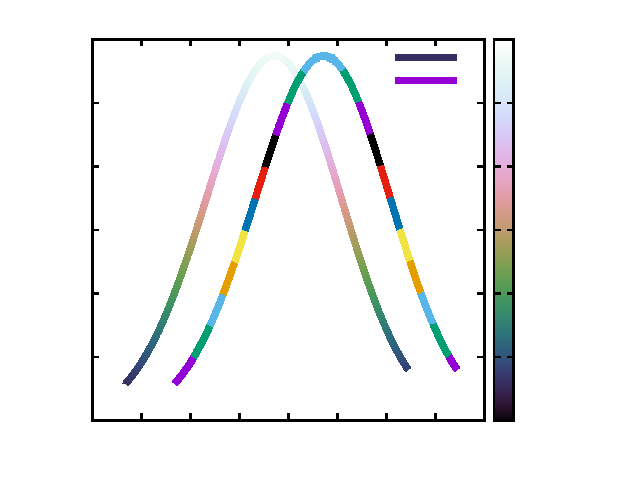
\includegraphics{figures/palette/plot}}%
    \gplfronttext
  \end{picture}%
\endgroup

    % }
\end{center}
\end{frame}

\begin{frame}{More info}
    \begin{itemize}
        \item The \texttt{help} command has a lot of information
        \item Lots of demos \url{http://gnuplot.sourceforge.net/demo_5.2/}
    \end{itemize}
\end{frame}

\end{document}
 
